\documentclass[12pt, english, a4paper]{report}
\usepackage{babel}
\usepackage{microtype}
\usepackage{graphicx}
\usepackage{fancyhdr}
\usepackage{geometry}
\usepackage{abstract}
\usepackage{titlesec}
\usepackage{enumitem}
\usepackage{multirow}
\usepackage{listings}
\usepackage{csquotes}
\usepackage{xcolor}
\usepackage{xurl}
\usepackage{hyperref}
\usepackage{float}
\usepackage{caption}
\usepackage{pdfpages}
\usepackage{nimbusmono}
\usepackage{nimbussans}
\usepackage[T1]{fontenc}
\usepackage{amsmath}
\usepackage{amsfonts}
\usepackage{cleveref}
\usepackage{booktabs}


%generates filler text
\usepackage{lipsum}

\usepackage[style=ieee,backend=bibtex,sorting=none]{biblatex}

\addbibresource{bibliography.bib}

\newcommand{\university}{Politehnica University of Timișoara}
\newcommand{\studyProgram}{Computers and Information Technology}
\newcommand{\academicYear}{2025}
\newcommand{\monthOfPresentation}{June}
\newcommand{\firstName}{Virgil-Alexandru}
\newcommand{\lastName}{Crișan}
\newcommand{\thesisTitle}{PiIrrigate: A Smart Irrigation System}
% Asist.(SL/Lect./Conf./Prof.)dr.ing.(arh./ec./chim.)
\newcommand{\coordinatorTitle}{Conf. dr. ing.}
\newcommand{\coordinatorFirstName}{Răzvan}
\newcommand{\coordinatorLastName}{Bogdan}
\newcommand{\declarationPath}{example_declaration.pdf}

\newcommand{\candidateName}{\firstName{} \MakeUppercase{\lastName}}
\newcommand{\coordinator}{\coordinatorTitle{} \coordinatorFirstName{} \MakeUppercase{\coordinatorLastName}}
% set document margins
\geometry{
 left=20mm,
 right=20mm,
 top=25mm,
 bottom=20mm,
 headheight=21mm,
 headsep=4mm
 }
 
 % set Nimbus Sans as default font - it is similar to Arial and Helvetica
 % Arial is proprietary and it doesn't work with diacritics
\renewcommand*\familydefault{\sfdefault}
\linespread{1.15} 
\setlength{\parindent}{1.5cm}

% Link border style
\hypersetup{
    pdfborderstyle={/S/U/W 1}, % underline links instead of boxes
    linkbordercolor=red,       % color of internal links
    citebordercolor=green,     % color of links to bibliography
    filebordercolor=orange,   % color of file links
    urlbordercolor=blue        % color of external links
}

\lstset{
	numbers=left, 
	numberstyle=\tiny, 
	numbersep=5pt,
	belowcaptionskip=1\baselineskip,
	breaklines=true,
	frame=l,
	xleftmargin=0.1\textwidth,
	showstringspaces=false,
	basicstyle=\footnotesize\ttfamily,
	keywordstyle=\bfseries\color{green!40!black},
	commentstyle=\itshape\color{purple!40!black},
	identifierstyle=\color{blue},
	stringstyle=\color{orange}
}

% Disable hyphenation
\pretolerance=10000
\tolerance=2000 
\emergencystretch=10pt

%\floatstyle{}
\newfloat{code}{h}{loc}[chapter]

% Set caption names
\setlocalecaption{english}{figure}{Figure}
\setlocalecaption{english}{table}{Table}
%\renewcommand{\lstlistingname}{Snippet}
\floatname{code}{Snippet}

%\renewcommand{\thelisting}{\thechapter.\arabic{listing}}
\setlength{\intextsep }{12pt plus 1pt minus 1pt} 

% Set citation names
\crefname{code}{Snippet}{Snippet}
\crefname{figure}{Figure}{Figure}
\crefname{table}{Table}{Table}
\crefname{equation}{}{}
\crefname{section}{Section}{Section}
\crefname{chapter}{Chapter}{Capter}
%\renewcommand*{\lstlistlistingname}{Snippet list}

% Make floats centered
\captionsetup{width=0.6\textwidth}

\makeatletter
\g@addto@macro\@floatboxreset\centering
\makeatother
\fancypagestyle{titlepagestyle}{
    \fancyhf{}
     \fancyhead[L]{
         \fontsize{8}{9.6}\selectfont
         \studyProgram \\
         \textbf{\academicYear} \\
     }
     \fancyhead[R]{
\includegraphics[height=15mm, keepaspectratio]{images/logo.png}}
    \fancyheadoffset[rh]{20mm}
    \renewcommand{\headrulewidth}{0pt}
    \renewcommand\footrulewidth{0pt}
}

\fancypagestyle{abstractpagestyle}{
    \fancyhf{}
    \fancyhead[L]{
    	\fontsize{8}{9.6}\selectfont
		\studyProgram{} \\
		\academicYear \\
		\candidateName{} \\
		\thesisTitle
    }
    \fancyhead[R]{
\includegraphics[height=15mm, keepaspectratio]{images/logo.png}}
    \fancyheadoffset[rh]{20mm}
    \renewcommand{\headrulewidth}{0pt}
    \renewcommand\footrulewidth{0pt}
}

\fancypagestyle{pagestyle}{
    \fancyhf{}
    \fancyhead[L]{
        \fontsize{8}{9.6}\selectfont
		\studyProgram{} \\
		\academicYear \\
		\candidateName{} \\
		\thesisTitle
    }
    \fancyhead[R]{
\includegraphics[height=15mm, keepaspectratio]{images/logo.png}}
    \fancyfoot[C]{- {\thepage} -}
    \fancyheadoffset[rh]{20mm}
    \renewcommand{\headrulewidth}{0pt}
    \renewcommand\footrulewidth{0pt}
}

\fancypagestyle{plain}{\pagestyle{pagestyle}}

% set chapter titles format
\titleformat
{\chapter}
[hang]
{\bfseries\fontsize{14pt}{18pt}\selectfont\MakeUppercase} % format
{\thechapter.}
{1em}
{\centering}

\titlespacing
{\chapter}
{0cm}
{0pt}
{24pt}

% set section titles format
\titleformat
{\section}
[hang]
{\bfseries\fontsize{12pt}{16pt}\selectfont\MakeUppercase} % format
{\thesection}
{1.5em}
{}

\titlespacing
{\section}
{0pt}
{12pt}
{12pt}

% set sub section titles format
\titleformat
{\subsection}
[hang]
{\fontsize{12pt}{16pt}\selectfont\MakeUppercase} % format
{\thesubsection}
{2em}
{}

\titlespacing
{\subsection}
{0pt}
{12pt}
{12pt}

\titleformat
{name=\chapter, numberless}
[hang]
{\bfseries\fontsize{14pt}{18pt}\selectfont\MakeUppercase}
{}
{0pt}
{\centering}%

\titlespacing
{name=\chapter, numberless}
{0pt}
{0pt}
{24pt}
%\setlength\cftaftertoctitleskip{8pt}

\begin{document}
\pagestyle{pagestyle}
\begin{titlepage}
\thispagestyle{titlepagestyle}
    \begin{center}
        \vspace*{\fill}
        \textbf{\fontsize{20pt}{30pt} \selectfont \MakeUppercase{\thesisTitle}}
    \end{center}
    
    \vspace*{\fill}
     
            
    \textbf{\fontsize{14pt}{16pt} \selectfont Candidate: \candidateName}
    
    \vspace{14pt}
    
    \textbf{\fontsize{14pt}{16pt} \selectfont Scientific coordinator: \coordinator}

    \begin{center}
        \vspace{50pt}
        \fontsize{14pt}{16pt} \selectfont Session: \monthOfPresentation{} \academicYear 
    \end{center}
    

\end{titlepage}
\thispagestyle{abstractpagestyle}

\vspace*{36pt}

\begin{center}
\textbf{\fontsize{20pt}{24pt} \selectfont REZUMAT}
\end{center}

\vspace{24pt}

Aceastăs lucrare descrie proiectarea și realizarea sistemului “PiIrrigate”. Acest sistem are ca scop eficientizarea consumului de apă si optimizarea culturilor agricole sau a grădinilor, prin utilizarea tehnologiilor moderne IoT și a comunicațiilor radio de tip LoRa. Pe măsură ce efectele încălzirii globale se fac din ce în ce mai resimțite, automatizarea si monitorizarea irigațiilor devine o necesitate. Proiectul vizează dezvoltarea unui sistem de monitorizare si control destinat fermierilor care doresc monitorizarea unor suprafețe mari de teren, dar acest sistem poate fi folosit si pentru sere inteligente  sau grădinărit normal.

\vspace{12pt}

Proiectul utilizează o arhitectură bazată pe microcontrolere Raspberry Pi și T-Beam LILYGO ESP32 LoRa. Aceste componente sunt folosite pentru colectarea si transmiterea datelor in timp real. Sistemul permite monitorizarea parametrilor esențiali (umiditate, temperatură, umiditatea solului și cantitatea de ploaie) prin senzori care sunt conectați la nodurile ESP32. Dupa colectare,  datele urmează a fi transmise către un gateway care comunică apoi cu un API web dezvoltat in .NET. Apoi datele urmează a fi stocate într-o baza de date PostgreSQL și trimise folosind SignalR către o aplicație web pentru a fi vizualizate în timp real de către utilizatori.

\vspace{12pt}
Utilizatorii au la dispoziție o interfață web care le permite atât vizualizarea datelor în timp real cât și vizualizarea datelor istorice și controlul manual al sistemului. De asemenea, acest sistem implementează un mecanism de înregistrare dinamica a nodurilor în rețea, lucru care permite extinderea facilă a sistemului.

\vspace{12pt}
Prin integrarea componentelor hardware și software într-o soluție coerentă, PiIrrigate demonstrează fezabilitatea și eficiența unui sistem IoT dedicat agriculturii inteligente, cu un impact potențial in reducerea consumului de apă și creșterea randamentului agricol.

\vfill
\thispagestyle{abstractpagestyle}

\vspace*{36pt}

\begin{center}
    \textbf{\fontsize{20pt}{24pt} \selectfont ABSTRACT}
\end{center}

\vspace{24pt}

This paper describes the design and implementation of the “PiIrrigate” system. The purpose of this system is to optimize water consumption and improve the management of agricultural crops or gardens by using modern IoT technologies and LoRa radio communications. As the effects of global warming become increasingly evident, the automation and monitoring of irrigation systems is becoming a necessity. The project aims to develop a monitoring and control system intended for farmers who need to oversee large areas of land, but it can also be used for smart greenhouses or regular gardening.
\vspace{12pt}

The project uses an architecture based on Raspberry Pi microcontrollers and T-Beam LILYGO ESP32 LoRa modules. These components are used for the real-time collection and transmission of data. The system enables the monitoring of essential parameters (humidity, temperature, soil moisture, and rainfall) through sensors connected to ESP32 nodes. After collection, the data is transmitted to a gateway, which then communicates with a web API developed in .NET. The data is stored in a PostgreSQL database and sent in real time via SignalR to a web application, where it can be viewed by users.
\vspace{12pt}
Users have access to a web interface that allows them to visualize both real-time and historical data, as well as to manually control the system. Additionally, the system implements a dynamic node registration mechanism, enabling easy expansion of the network.
\vspace{12pt}
By integrating both hardware and software components into a coherent solution, PiIrrigate demonstrates the feasibility and efficiency of an IoT-based system dedicated to smart agriculture, with the potential to reduce water consumption and increase agricultural productivity.
\vfill
\tableofcontents
\listoffigures
\vspace{24pt}
\begingroup
	\let\clearpage\relax
	\listoftables
	\vspace{24pt}
	\listof{code}{List of Snippets}
\endgroup
\chapter{Introduction}\label{section:introduction}
\thispagestyle{pagestyle}


\section{CONTEXT}

Agriculture is a vital sector that plays a crucial role in sustaining human life and the economy.
Agriculture automation and optimization has become a major concern in recent years. 
As the global population continues to grow, the demand for food is increasing and the developing need for food
along with the effect of climate changes are forcing the agricultural industry to adapt and innovate\cite{OBAIDEEN2022100124}.

In the last 35 years, the wold has seen a doubling of the agricultural production. This has been achieved throught the use
of different fertilizers, pesticides and herbicides. This doubling was associated with a 6.87-fold increase in nitrogen fertilization,
a 3.48-fold increase in phosphorus fertilization and 1.68-fold increase in the amount of irrigated cropland \cite{doi:10.1073/pnas.96.11.5995}.
In addition, the water consumoption is expected to increase by 50\% by 2050 \cite{s20236865}. 

This project aims to address the challenges of water scarcity and the need of efficient irrigation systems
by presenting the plan, the implementation, the results and future work of a system that can be used in different
scenarios and is meant to help reducing the water consumption and increasing the agricultural productivity.
The PiIrrigate project intends achuive this by developing an innovative irrigation system that leverages the power of 
IoT and LoRa radio communication technologies.  
The main focus of this project is to create a system that can be easly used in different agricultural settings, 
starting from small gardens to large farms and even smart greenhouses. Beside this, I wanted to create a system that 
is easy to use and can be extended with ease. 

The ESP32 boards with sensors are responsible for colecting the data. Then data is sent using  LoRa to another
ESP32 board that acts as a gateway connected to a Raspberry Pi, which is responsible for sending the data to a web API.
The web API is developed in .NET and is responsible for storing the data in a PostgreSQL database.
The data is then sent to a web application using SignalR, which allows real-time communication between the server and the client.
The web application is responsible for displaying the live data and the historical data and also for providing a way to
control the system manually and to add new nodes to the system. 

This system takes advantage of the LoRa radio communication technology, 
which allows for long-range communication with low power consumption. Meaning that the system can be used in remote areas and
it will work even if the internet connection is not available to all the nodes. The Raspberry Pi is the only component of this system
that needs to be connected to the internet. Other components can be scatered on a area of 10km or more, depending on
the environment and the node setup (mesh or star topology).

\newpage
\section{MOTIVATION}


The reason why I choose to create such a system was fulled by my passion for technology and smart agriculture. Besides this,
I like to observe the data path, from the moment it is collected by the sensors, to the moment it is displayed
in a web application. 
I have always been intested in pieces of technology that can be used to solve real world problems and now I had the chance
to create such a system.

Initially, I wanted to create a system for my own lawn, but as I started working on the project, I realized that the system
can be used in many other scenarios, such as smart greenhouses or even large farms or vineyards. 

\chapter{State of the Art}\label{section:stateoftheart}

\section{Introduction}
The state of the art chapter provides an overview of the current state of smart irrigation 
systems and their applications in agriculture. 
This chapter will explore the existing technologies, methods, and solutions used in smart irrigation. 
It will also highlight the gaps and challenges in the current systems,
and how the PiIrrigate project aims to address these issues.

\section{Existing Smart Irrigation Solutions}
\subsection{Types of Smart Irrigation Systems}

There are several types of smart irrigation systems used in modern agriculture:

\begin{itemize}
  \item \textbf{Weather-Based Controllers} \\
  These systems use weather data to adjust irrigation schedules based on evapotranspiration rates, 
  ensuring that plants receive the right amount of water.

  \item \textbf{Soil Moisture-Based Controllers} \\
  These systems rely on data from soil moisture sensors placed in the root zone of the plants.
  Irrigation cycles are triggered when the soil moisture drops below a predetermined threshold, 
  ensuring plants receive water only when necessary.
  This method is very precise for specific zones\cite{smartIrrigationTechnologyControllersAndSensors}.

  \item \textbf{Hybrid Systems} \\
  Many modern systems utilize a hybrid approach, combining data from both
  weather feeds and soil moisture sensors for more accurate and resilient 
  irrigation decisions. Some research also explores "hybrid" in terms of 
  integrating different energy sources (e.g., solar and wind) to power the systems or 
  combining various 
  irrigation methods (like drip and sprinkler) under one smart control\cite{soilBasedIrrigation}.

  The PiIrrigate project place itself in the category of hybrid systems, using both
  soil moisture sensors and weather sensors to collect data.
  
  Some of the most popular hybrid smart irrigation systems include:
  \begin{itemize}
    \item \textbf{Netafim's Precision Irrigation System} \\
    This system cobines data from soil moisture and flow sensors with sattelite weather data and predictive
    analytics to optimize the irrigation proccess.
    
    Key features include:
    \begin{itemize}
      \item Real-time monitoring of soil moisture levels and weather forecasts.
      \item Automated irrigation scheduling based on weather forecasts.
      \item AI-based algorithms to optimize the irrigation timing and duration.
    \end{itemize}

    \item \textbf{CropX Smart Farming System} \\
    CropX is a cloud based platform that integrates soil moisture sensors, weather data and
    machine learning algorithms to optimize the irrigation process.

    Key features include:
    \begin{itemize}
      \item Irrigation recomandations based on soil variability, crop type and weather.
      \item Farmers can apply recommandations or integrate with automated irrigaitons contrllers.
      \item Easy to scale and adapt to different farm sizes from small to large-scale farms.
    \end{itemize}
  
    \item \textbf{Toro EVOLUTION® Series Controller with Smart ET Sensor} \\
    Combines basic sprinkler system hardware with smart sensors and connectivity,
    offering both manual and intelligent irrigation options. The evaporation sensors are used to measure
    the amount of water lost throught evaporation and adjust the irrigation accordingly.

    Key features include:
    \begin{itemize}
      \item Can be programmed manually or connected to a local weather station.
      \item Smart ET sensor measures evaporation rates and adjusts irrigation schedules.
      \item Compatible with smart devices for remote monitoring
    \end{itemize}
  \end{itemize}
\end{itemize}

\section{Comparative Analysis of Smart Irrigation Systems}
The table below provides a comparative analysis of some of the most popular smart 
irrigation systems available today and the PiIrrigate system.

\begin{table}[ht]
\centering
\begin{tabular}{|p{3.2cm}|p{3.2cm}|p{3.2cm}|p{3.2cm}|p{3.2cm}|}
\hline
\textbf{Feature} & \textbf{Netafim} & \textbf{CropX} & \textbf{Toro ET} & \textbf{PiIrrigate} \\
\hline
Irrigation Type & Drip & Any & Sprinkler & Custom \\
\hline
Automation & High (AI) & Med–High & Medium & Medium \\
\hline
Sensors & Soil, flow, weather & Soil, temp & ET sensor & Soil, temp, rain \\
\hline
Weather Data & Yes & Yes & Yes & Optional \\
\hline
Manual Control & App/cloud & App/web & Panel/app & Web UI \\
\hline
AI/Analytics & Yes & Yes & No & No \\
\hline
Scalability & Large farms & Small–large & Residential & Small farms/gardens \\
\hline
Cloud Sync & Yes & Yes & Optional & Yes \\
\hline
Use Case & Precision agri & Smart farming & Lawn care & Small to large scale\\
\hline
Cost & High & Med–High & Low–Mid & Low \\
\hline
\end{tabular}
\caption{Comparison of Smart Irrigation Systems}
\label{tab:irrigation_comparison}
\end{table}

\section{Identified Gaps and Challenges}
Despite the advancements in smart irrigation systems, several gaps and challenges remain:

\begin{itemize}
  \item \textbf{High Costs} \\
  Many existing systems are expensive, making them inaccessible for small farmers or home gardeners.
  
  \item \textbf{Complexity of Use} \\
  Some systems require specialized knowledge to set up and maintain, which can be a barrier for adoption.

  \item \textbf{Limited Customization} \\
  Many systems are designed for specific crops or environments, limiting their applicability in diverse agricultural settings.

  \item \textbf{Data Integration Issues} \\
  Integrating data from multiple sources (e.g., weather, soil sensors) can be challenging, leading to inefficiencies in irrigation management.
\end{itemize}

Bedside the presented gaps, there are also some other challenges that need to be addressed, such as:
data security and privacy concerns, the need for reliable internet connectivity in remote areas, 
and the need for systems that can operate in harsh environmental conditions. 

Another aspect that needs to be considered is the environmental impact of smart irrigation systems.
While these systems are designed to optimize water usage,
the production and disposal of electronic components can have a negative impact on the environment.
So another challenge is to create systems that are environmentally friendly and sustainable. This means 
that the components used in these systems shlould be madea from recyclable materials 
and the systems should be designed to have a long lifespan and to be easily repairable.

\section{Summary}
In summary, the state of the art in smart irrigation systems shows significant 
advancements in technology and methods, but also highlights several gaps and challenges 
that need to be addressed. The PiIrrigate project aims to fill these gaps by providing a
cost-effective, easy-to-use, and customizable solution that leverages the power of IoT and LoRa 
radio communication technologies. 

\chapter{Used Technologies}
\section{Development Process Tools}
\subsection{Version Control: GitHub}
GitHub is a web-based platform that uses Git for version control and collaboration on software projects.
It enables developers to collaborate in real-time. Thhey can track changes, manage issues, and review code.
It was released in 2008 and in 2018 it was acquired by Microsoft\cite{githubDefinition}.
Github is widely used in the software development industry and in has become standard practice to 
use GitHub for version control. 

\subsection{Software Development: Visual Studio Code and Visual Studio}
Visual Studio Code (VS Code) is a free lightweight code editor developed by Microsoft.
It supports a wide range of programming langueges and has a rich collection of extensiont that can be used to 
enchance its functionality.
It was very convinient to use a single code editor for multiple programming languages and frameworks.
To be more specific, I used Visual Studio Code for ESP32 programming, along with Platform IO, 
which is an open-source ecosystem for IoT development. VSCode was also used for the Angular web application 
development. The Raspberry Pi was programmed using Python, I used Visual Studio Code and for remote access
I used SSH.

Visual Studio is a more comprehensive integrated development environment (IDE) that provides advance features
for software development, such as debugging, profiling, and testing.
Visual Studio is also developed by Microsoft and it is widely used in the software development industry.
Since the PiIrrigate's web API was developed in .NET, I used Visual Studio for the API development.

\subsection{System Architecture: Draw.io}
Draw.io is a free online diagramming tool that allows users to create flowcharts, 
UML diagrams, network diagrams, and more. 
Other alternatives include Lucidchart, Microsoft Visio, and Gliffy. But I found that Draw.io is easy to use
and provides a wide range of templates and shapes that can be used to create diagrams.

\subsection{Iot Device Management: Azure IoT Hub}
Azure IoT Hub is a cloud-based service that enables secure and reliable 
communication between IoT devices and the cloud.
It provides a way to connect, monitor, and manage IoT devices at scale.
Azure IoT Hub is used in the PiIrrigate project to manage the
communication between the Raspberry Pi and the web API.

\section{Communication Technologies}
\subsection{LoRa Radio Communication}
LoRa is a wireless modulation technique derived from Chirp Spread Spectrum (CSS) technology.
LoRa modulated transmission is robust against disturbances and can be received across great distances.
It has become popular, as one of the most used standards for device interconnection, mainly because of its
low power consumption and long-range capabilities\cite{lora}. This technology was used in the PiIrrigate project
to enable the communication between the ESP32 nodes and the ESP32 gateway connected to the Raspberry Pi.

\subsection{MQTT Protocol}
MQTT (Message Queuing Telemetry Transport) is a 
an OASIS standard lightweight messaging protocol for the Internet of Things (IoT).
It is designed as an extremely lightweight publish/subscribe messaging transport that is ideal for connecting 
remote devices with a small code footprint and minimal network bandwidth. 
In the PiIrrigate project, MQTT is used to send data from the Raspberry Pi to IoTHub
and from the web API to the web application.

\subsection{HTTP Protocol}
HTTP is an application layer protocol for transmitting hypermedia documents, such as HTML.
It was designed for communication between web browsers and servers, 
but it can also be used for machine-to-machine communication.
In the PiIrrigate project, HTTP is used to send data from the web API to the web application\cite{http}.

\subsection{SignalR and WebSockets}
SignalR is an open-source library for ASP.NET that simplifies 
the process of adding real-time web functionality to applications.
It allows server-side code to push content to connected clients instantly as it becomes available.
SignalR uses WebSockets as its primary transport protocol, but it can also fall back to other techniques like
Server-Sent Events or Long Polling if WebSockets are not available.
In the PiIrrigate project, SignalR is used to provide real-time communication 
between the web API and the web application.

\section{Programming Languages and Frameworks}
\subsection{C\# and .NET}
C\# is a modern, object-oriented programming language developed by Microsoft.
It is widely used for developing Windows applications, web applications, and cloud services.
.NET is a free, open-source developer platform that provides a wide range of tools and libraries 
for building applications.
In the PiIrrigate project, C\# and .NET are used to develop the web API that manages the communication
between the Raspberry Pi and the web application, as well as to handle data storage in the PostgreSQL database.

\subsection{Entity Framework Core}
Entity Framework Core (EF Core) is an open-source, lightweight, extensible, and cross-platform version 
of the Entity Framework, which is an object-relational mapper (ORM) for .NET.
EF Core allows developers to work with databases using .NET objects, eliminating the need for 
most of the data access code that developers usually need to write.
In the PiIrrigate project, EF Core is used to interact with the PostgreSQL database,

\subsection{Python}
Python is a high-level, interpreted programming language known for its simplicity and readability.
It is widely used in various domains, including web development, data analysis, machine learning, and IoT.
In the PiIrrigate project, Python is used to develop the code that runs on the Raspberry Pi,
which is responsible for receiving data from the ESP32 nodes and sending it to the web API.

\subsection{Arduino C/C++}
Arduino C/C++ is a simplified version of C/C++ that is used to program Arduino 
boards and other microcontrollers.
It provides a set of libraries and functions that make it easy to interact with hardware components.
In the PiIrrigate project, Arduino C/C++ is used to program the ESP32 nodes that collect data from the sensors
and send it to the gateway using LoRa radio communication.

\subsection{Angular and TypeScript}
Angular is a platform and framework for building single-page client applications using HTML and TypeScript.
It is developed and maintained by Google and is widely used for building modern web applications.
In the PiIrrigate project, Angular is used to develop the web application that provides a user interface for
monitoring and controlling the irrigation system.

TypeScript is a superset of JavaScript that adds static typing and other features to the language.
It is designed for large-scale applications and provides better tooling and error checking compared to JavaScript.
JavaScript is a high-level, interpreted programming language that is widely used for building web applications.
It is primarly used for client-side scripting, but it can also be used for
 server-side development using Node.js.

\chapter{PiIrrigate System Overview}\label{section:overview}

\section{Overview}
The Internet of Things (IoT) is a new technology that allows devices to connect remotely to achieve smart
farming \cite{agriculture12101745}. The IoT has a wide range of applications in agriculture, and it has 
began to influence many other industries as well, such as healthcare, transportation, and manufacturing. 
This was done to improve the efficiency and productivity of these industries, 
as well as to reduce costs and improve the quality of products and services\cite{s19081833}.

The PiIrrigate smart irrigation system is build using a combination of hardware and software technologies.
It leverages both low-power edge devices and cloud-based infrastructure to provide real-time monitoring
and data collection, as well as remote control capabilities.
The core components and their roles in the system are as follows:
\begin{itemize}
  \item \textbf{ESP32 (LilyGo T-Beam)} \\
  The LilyGo T-Beam is a development board based on the ESP32 microcontroller, it is equipped with
  LoRa radio communication capabilities, Wifi, Bluetooth, GPS, and a battery management system.
  It is used to collect data from sensors and send it to the gateway using LoRa radio communication.

  \item \textbf{Raspberry Pi} \\
  Raspberry Pi is a small, affordable computer that can be used for a wide range of applications.
  The Raspberry Pi is the core of the PiIrrigate irrigation module, 
  it is responsible for receiving data from the ESP32 nodes and sending it to Azure IoT Hub.

  \item \textbf{Azure IoT Hub} \\
  Azure IoT Hub is a cloud-based service that enables secure and reliable communication 
  between IoT devices and the cloud.
  It manages the bidirectional communication between the Raspberry Pi and the web API.

  \item \textbf{Web API} \\
  The web API is developed in .NET and is responsible for receiving data from the Raspberry Pi,
  storing it in a PostgreSQL database, and providing a way to access the data.
  SignalR is used to provide real-time communication between the server and the client.
  It also provides a way to control the system manually and to add new nodes to the system.

  \item \textbf{PostgreSQL Database} \\
  PostgreSQL is a powerful, open-source relational database management system.
  It is used to store the data collected from the sensors and the schedules sent to the system. It also
  stores the user data and the configuration of the system. The database is hosted in Neon.

  \item \textbf{Web Application} \\
  The web applicaiton is developed using Angular and is responsible for displaying live, historical data
  and provide the user interface for controlling the system.
\end{itemize}

In the following sections, we will explore each of these components in more detail,
starting with the hardware components and then moving on to the software components.

\section{Hardware Components}
\subsection{Sensors}
The PiIrrigate system uses a variety of sensors to collect data from the environment.
The sensors used in the PiIrrigate system are:
\begin{itemize}
  \item \textbf{Soil Moisture Sensor} \\
  The soil moisture sensor is used to measure the moisture level in the soil. It is used to determine when to irrigate the plants.
  The sensor is connected to the ESP32 board and sends the data to the gateway using LoRa radio communication.

  \item \textbf{Temperature and Humidity Sensor} \\
  The temperature and humidity sensor is used to measure the temperature and humidity of the environment.
  It is used to determine the optimal conditions for plant growth and to adjust the irrigation schedule accordingly.

  \item \textbf{Rain Sensor} \\
  The rain sensor is used to detect rain and prevent irrigation during rainy weather. 
  It helps to conserve water and prevent over-irrigation.
\end{itemize}
\subsection{ESP32 (LilyGo T-Beam)}

The T-Beam ESP32 LoRa Wireless Module is a compact development board thaht combines an ESP32 microcontroller,
LoRa transceiver (SX1278), GPS module, and a battery management system into a single unit. This board is ideal
for long-range, low-power IoT applications such as mesh networks, asset tracking, smart agriculture and environmental
monitoring. Besides this, it has a built-in OLED display. The communication range of the LoRa transceiver can reach up to 10 km in open areas.
\begin{figure}[H]
    \centering
    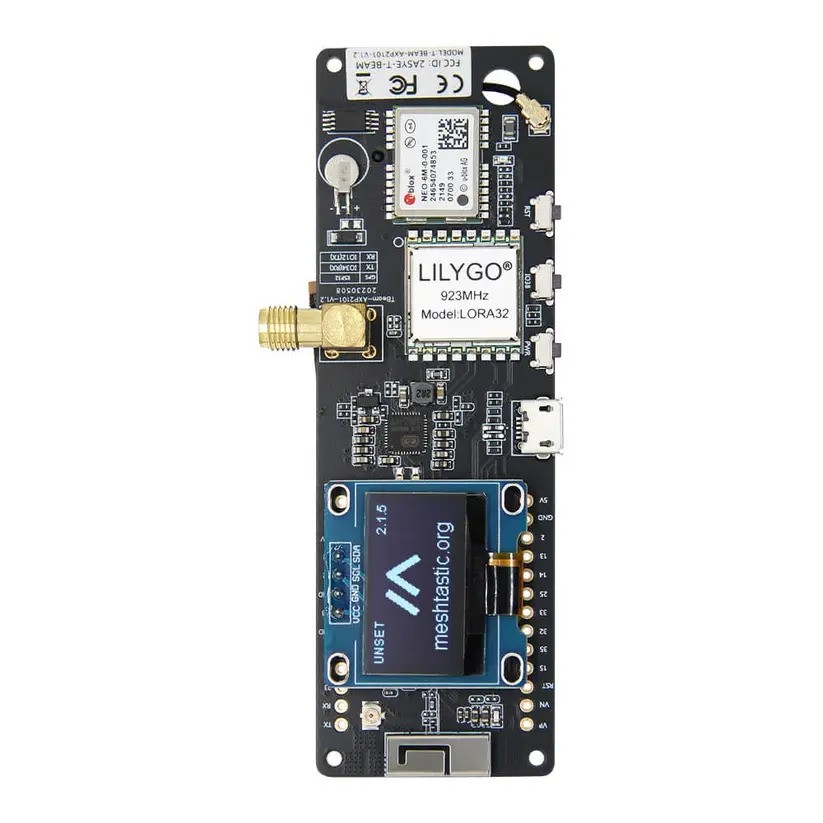
\includegraphics[width=0.8\textwidth]{images/esp32lora.jpg}
    \caption{ESP32 (LilyGo T-Beam) module used in PiIrrigate}
    \label{fig:esp32lora}
\end{figure}

\subsection{Raspberry Pi 4 Model B}
The Raspberry Pi 4 Model B is a small, affordable computer that can be used for a wide range of applications.
It is equipped with a quad-core ARM Cortex-A72 processor, up to 8GB of RAM, and supports dual-band Wi-Fi and Bluetooth.
The Raspberry Pi 4 Model B together with an ESP32LoRa is used in the PiIrrigate project as the gateway that receives data from the ESP32 nodes
and sends it to IoT Hub.
\begin{figure}[H]
    \centering
    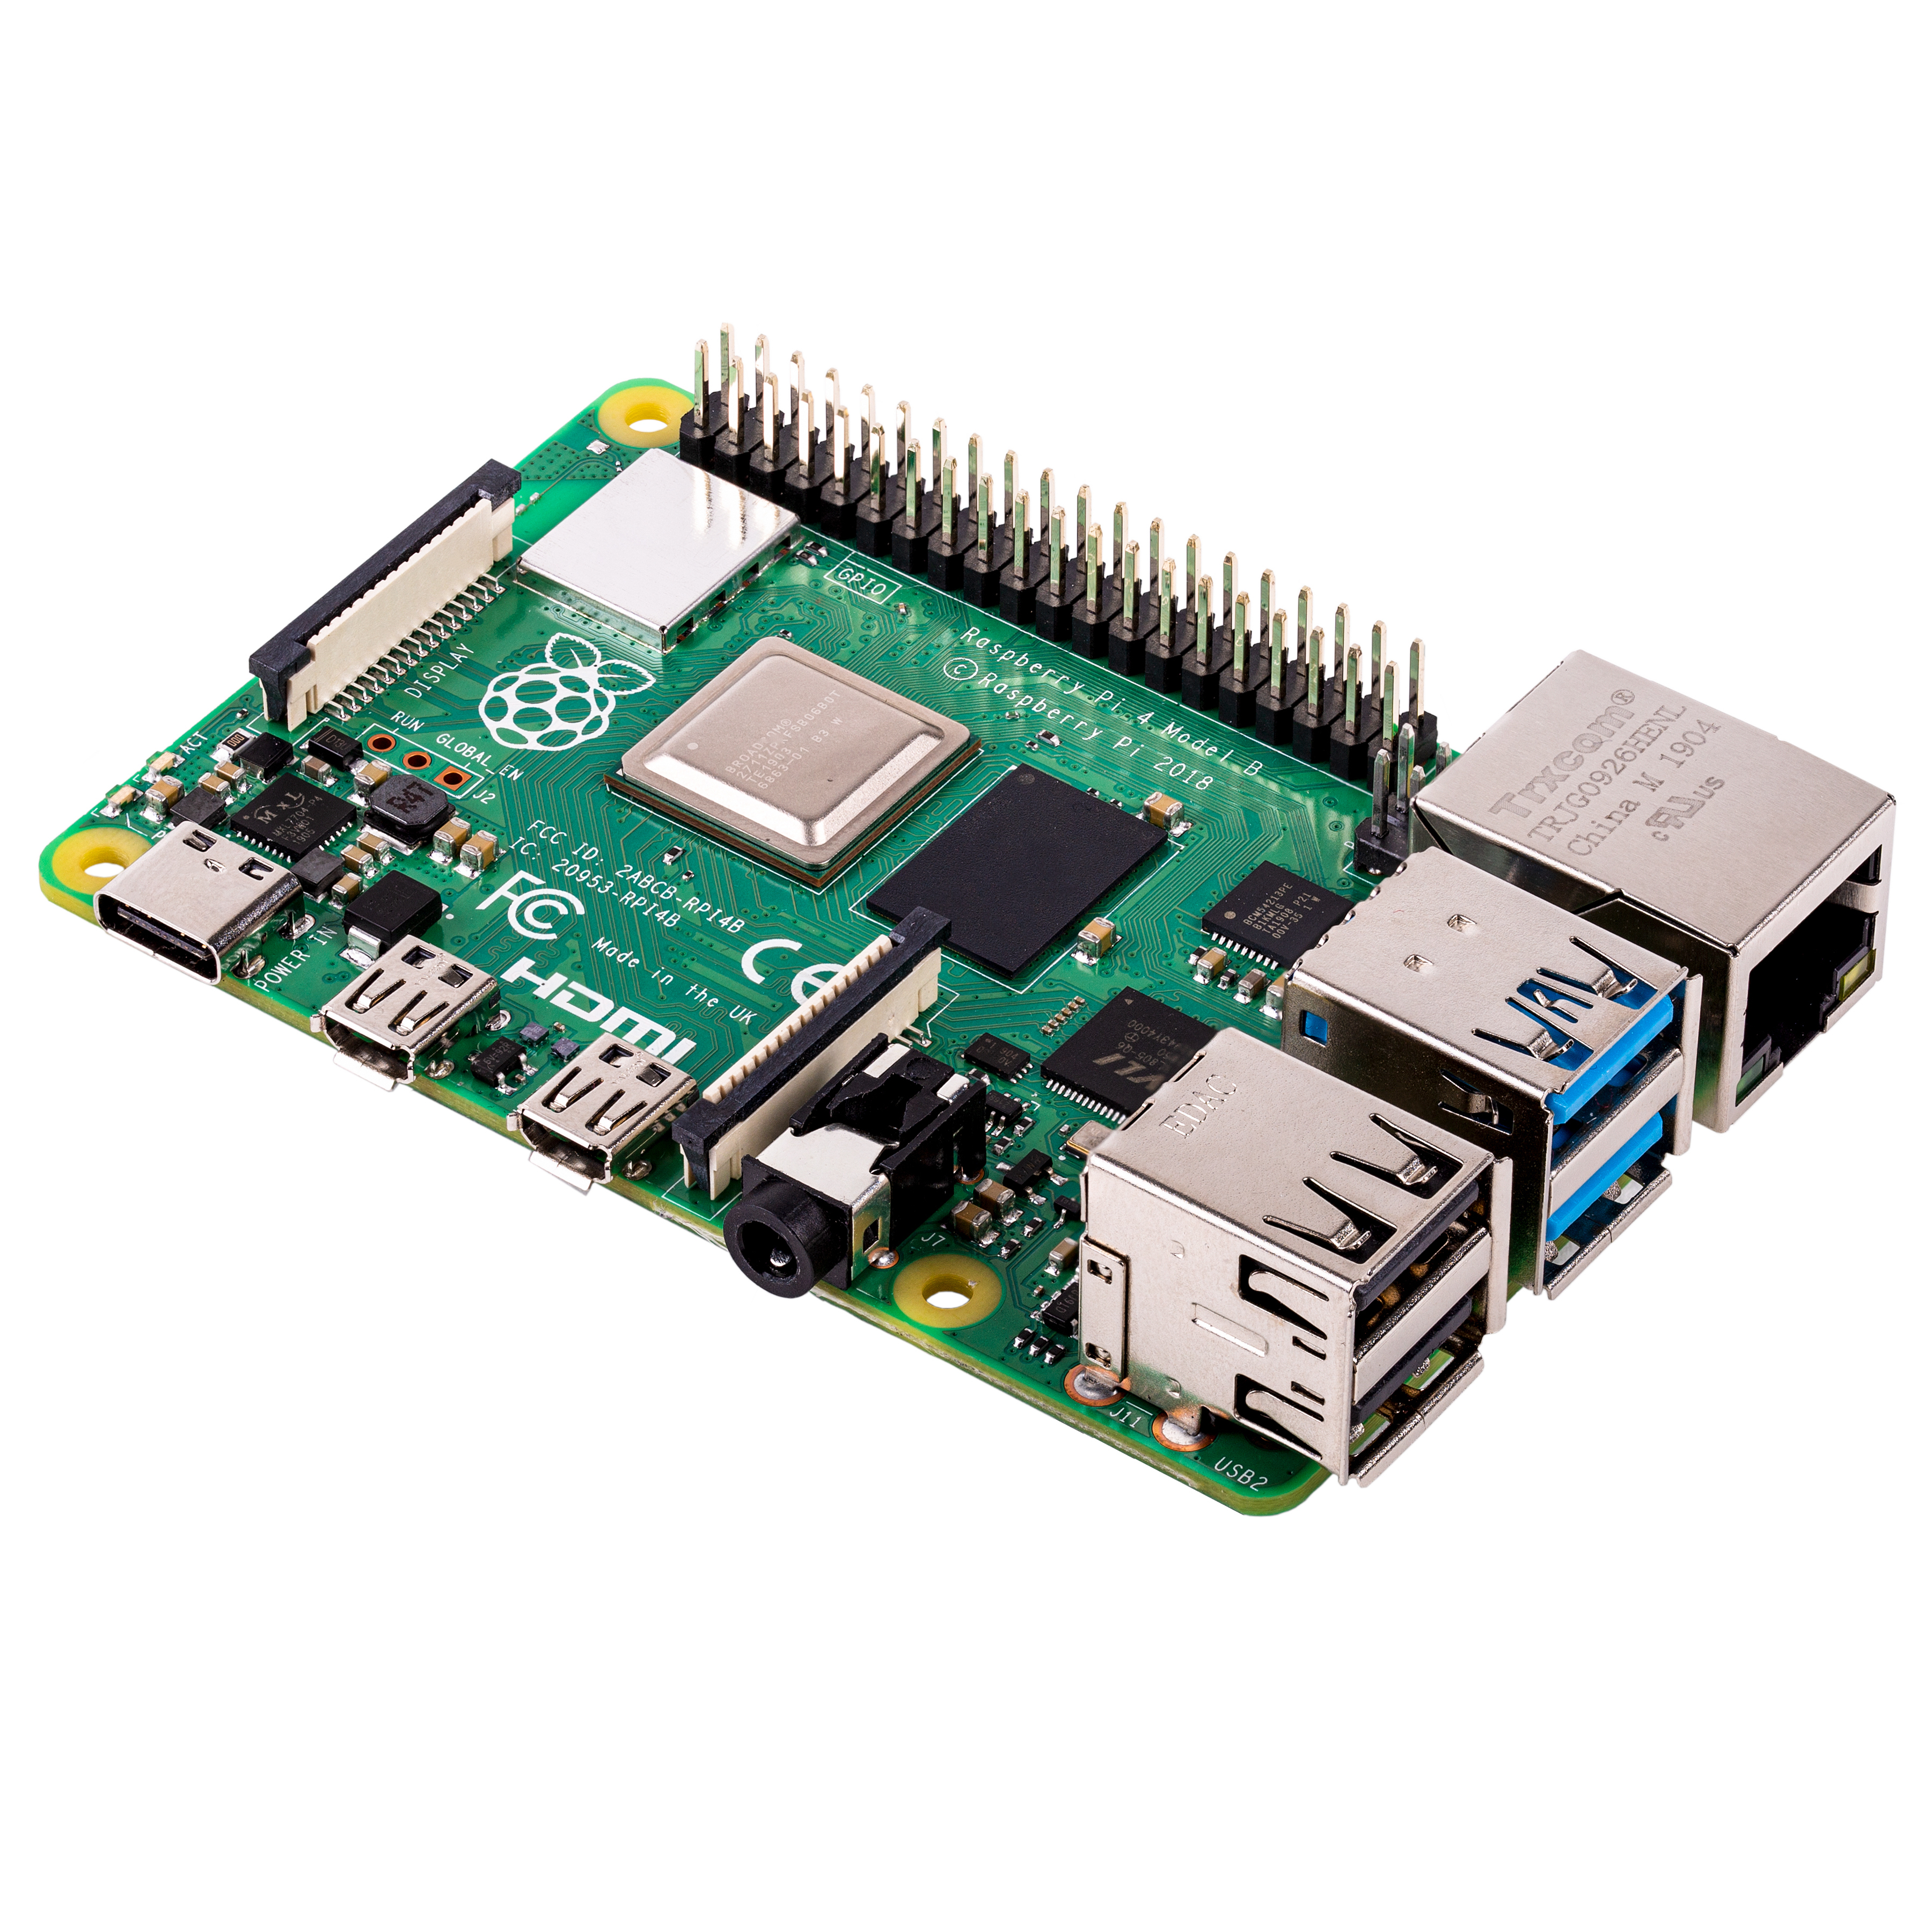
\includegraphics[width=0.8\textwidth]{images/raspberrypi.jpg}
    \caption{Raspberry Pi 4 Model B used in PiIrrigate}
    \label{fig:raspberrypi}
\end{figure}

\section{Data Flow}
The data flow in the PiIrrigate system is as follows:

\begin{enumerate}
  \item The ESP32 nodes collect data from the sensors and send it to the gateway using LoRa radio communication.
  \item The Raspberry Pi receives the data from the ESP32 nodes and sends it to Azure IoT Hub using MQTT protocol.
  \item The web API receives the data from Azure IoT Hub and stores it in the PostgreSQL database using Entity Framework Core. 
  \item The web application retrieves the data from the web API and displays it to the user in real-time using SignalR.
\end{enumerate}
\begin{figure}[H]
    \centering
    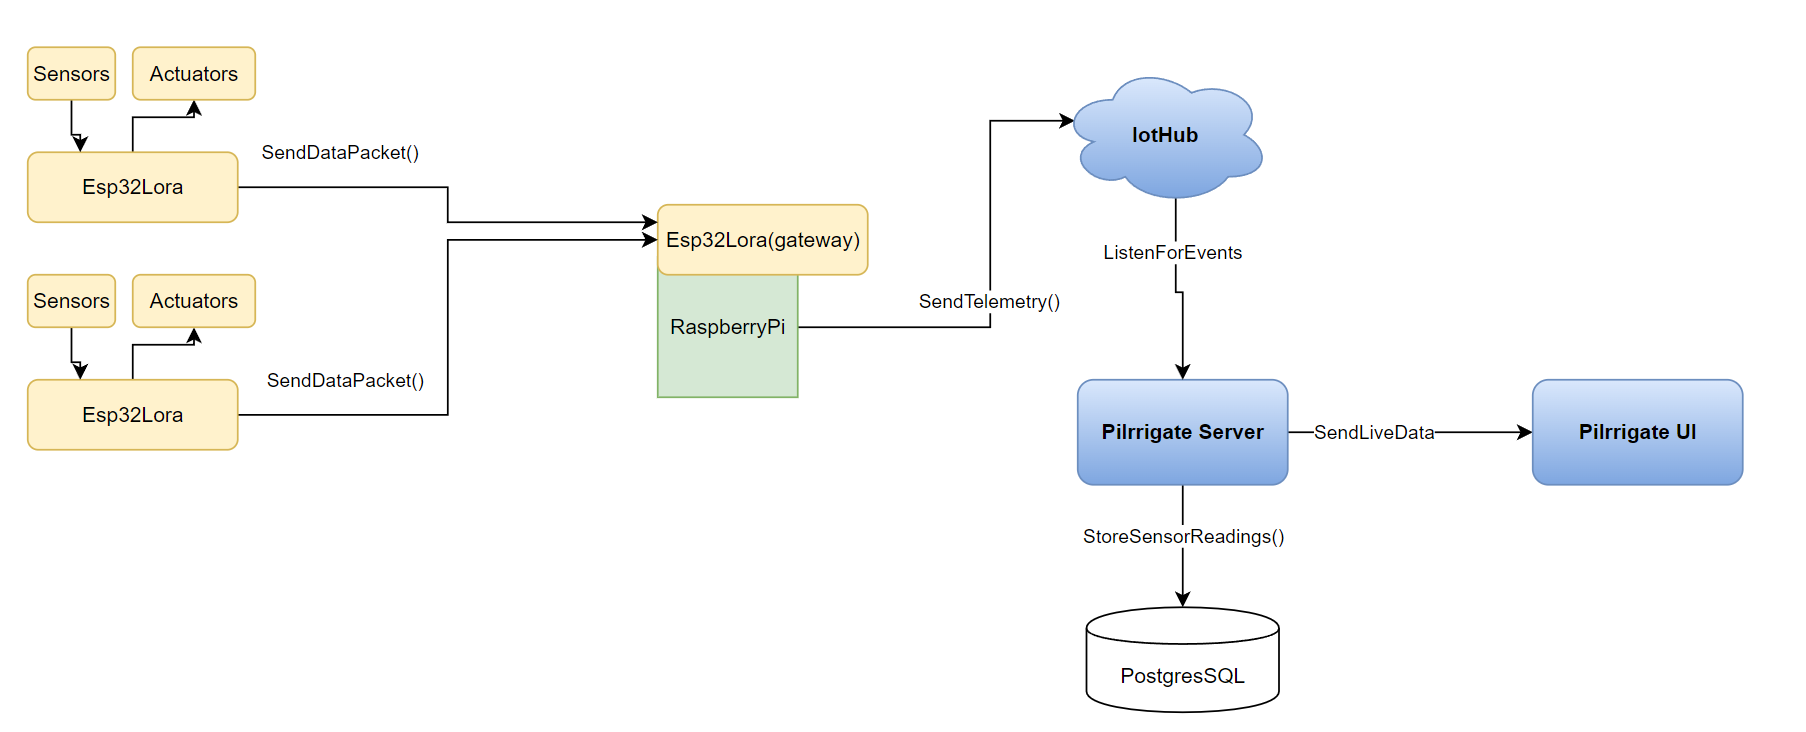
\includegraphics[width=0.8\textwidth]{images/system.png}
    \caption{PiIrrigate System overview}
    \label{fig:system-overview}
\end{figure}

\subsection{Data aquisition}
The data acquisition is done using the ESP32 nodes that collect data from the sensors.
For each sensor type, I created a specific library thath can be used to read the data from the sensor.
Temperature and humidity data is collected using a DHT11 sensor. The communication with the sensor is done using
1-wire digital interface. The communication is done in 3 steps\cite{1wire}:
\begin{enumerate}
  \item The microcontroller initiates communication by sending the start signal.
  The start signal is an 18\,ms LOW signal followed by a $20$--$40\,\mu$s HIGH signal.
  \item The sensor responds a fixed LOW and HIGH handshake pattern, indicating that it is ready to send data.
  Usually the acknowledgment is a $80\,\mu$s LOW signal followed by a $80\,\mu$s HIGH signal.
  \item After the handshake, the sensor sends a 40-bit data stream, which includes the humidity and temperature data.
  The bits are sent in a specific order: first the humidity data (16 bits), 
  then the temperature data (16 bits), 
  and finally a checksum (8 bits).
  Each bit is sent as a $50\,\mu$s LOW signal followed by a HIGH signal that lasts for either $26$--$28\,\mu$s (for a 0 bit) or $70\,\mu$s (for a 1 bit).
  In code, for each bit, the microcontroller waits for the LOW signal to start, 
  then waits for $30\,\mu$s then ig the signal is HIGH, the bit is a 1, otherwise it is a 0.
  The checksum is used to verify the integrity of the data received from the sensor.
\end{enumerate}

\begin{figure}[H]
    \centering
    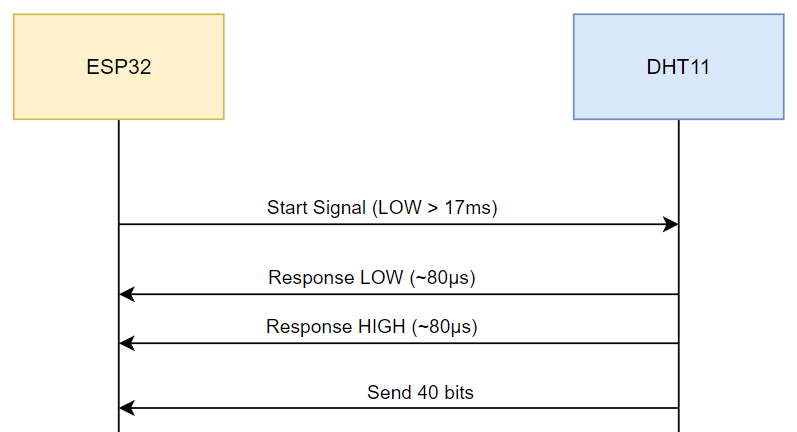
\includegraphics[width=0.8\textwidth]{images/dht-steps.png}
    \caption{Steps in data aquisition from DHT11 sensor}
    \label{fig:dht-steps}
\end{figure}
\chapter{State of the Art}\label{section:stateoftheart}

\section{Introduction}
The state of the art chapter provides an overview of the current state of smart irrigation 
systems and their applications in agriculture. 
This chapter will explore the existing technologies, methods, and solutions used in smart irrigation. 
It will also highlight the gaps and challenges in the current systems,
and how the PiIrrigate project aims to address these issues.

\section{Existing Smart Irrigation Solutions}
\subsection{Types of Smart Irrigation Systems}

There are several types of smart irrigation systems used in modern agriculture:

\begin{itemize}
  \item \textbf{Weather-Based Controllers} \\
  These system take advantage of available weather data, such as temperature, 
  humidity, and rainfall forecasts, to optimize irrigation schedules. This is not the
  most precise method as it does not use data from the soil, but it represent a good alternative
  for large areas.

  \item \textbf{Soil Moisture-Based Controllers} \\
  Soil moisture based controllers use sensors that are placed in the soil to measure
  the moisture level and adjust the irrigation accordingly.
  These are more precise than weather-based controllers, as they take into account
  the actual moisture level in the soil, but they require more maintenance and calibraiton
  \cite{smartIrrigationTechnologyControllersAndSensors}.

  \item \textbf{Hybrid Systems} \\
  Many modern systems utilize a hybrid approach, combining data from both
  weather feeds and soil moisture sensors for more accurate and resilient 
  irrigation decisions. Some research also explores "hybrid" in terms of 
  integrating different energy sources (e.g., solar and wind) to power the systems or 
  combining various 
  irrigation methods (like drip and sprinkler) under one smart control\cite{soilBasedIrrigation}.

  The PiIrrigate project place itself in the category of hybrid systems, using both
  soil moisture sensors and weather sensors to collect data.
  
  Some of the most popular hybrid smart irrigation systems include:
  \begin{itemize}
    \item \textbf{Netafim's Precision Irrigation System} \\
    This system cobines data from soil moisture and flow sensors with sattelite weather data and predictive
    analytics to optimize the irrigation proccess.
    
    Key features include:
    \begin{itemize}
      \item Real-time monitoring of soil moisture levels and weather forecasts.
      \item Automated irrigation scheduling based on weather forecasts.
      \item AI-based algorithms to optimize the irrigation timing and duration.
    \end{itemize}

    \item \textbf{CropX Smart Farming System} \\
    CropX is a cloud based platform that integrates soil moisture sensors, weather data and
    machine learning algorithms to optimize the irrigation process.

    Key features include:
    \begin{itemize}
      \item Irrigation recomandations based on soil variability, crop type and weather.
      \item Farmers can apply recommandations or integrate with automated irrigaitons contrllers.
      \item Easy to scale and adapt to different farm sizes from small to large-scale farms.
    \end{itemize}
  
    \item \textbf{Toro EVOLUTION® Series Controller with Smart ET Sensor} \\
    Combines basic sprinkler system hardware with smart sensors and connectivity,
    offering both manual and intelligent irrigation options. The evaporation sensors are used to measure
    the amount of water lost throught evaporation and adjust the irrigation accordingly.

    Key features include:
    \begin{itemize}
      \item Can be programmed manually or connected to a local weather station.
      \item Smart ET sensor measures evaporation rates and adjusts irrigation schedules.
      \item Compatible with smart devices for remote monitoring
    \end{itemize}
  \end{itemize}
\end{itemize}

\section{Comparative Analysis of Smart Irrigation Systems}
The table below provides a comparative analysis of some of the most popular smart 
irrigation systems available today and the PiIrrigate system.

\begin{table}[ht]
\centering
\begin{tabular}{|p{3.2cm}|p{3.2cm}|p{3.2cm}|p{3.2cm}|p{3.2cm}|}
\hline
\textbf{Feature} & \textbf{Netafim} & \textbf{CropX} & \textbf{Toro ET} & \textbf{PiIrrigate} \\
\hline
Irrigation Type & Drip & Any & Sprinkler & Custom \\
\hline
Automation & High (AI) & Med–High & Medium & Medium \\
\hline
Sensors & Soil, flow, weather & Soil, temp & ET sensor & Soil, temp, rain \\
\hline
Weather Data & Yes & Yes & Yes & Optional \\
\hline
Manual Control & App/cloud & App/web & Panel/app & Web UI \\
\hline
AI/Analytics & Yes & Yes & No & No \\
\hline
Scalability & Large farms & Small–large & Residential & Small farms/gardens \\
\hline
Cloud Sync & Yes & Yes & Optional & Yes \\
\hline
Use Case & Precision agri & Smart farming & Lawn care & Small to large scale\\
\hline
Cost & High & Med–High & Low–Mid & Low \\
\hline
\end{tabular}
\caption{Comparison of Smart Irrigation Systems}
\label{tab:irrigation_comparison}
\end{table}

\section{IoT and LoRa in Agriculture}
Agriculture is one of the biggest industries, critical to the global economy and food security. With the increasing food 
demant, the need for efficient and sustainable agricultural has grown in the last years. The IoT (Internet of Things) is
is a key technology that can help to address these challenges by providing real-time data and 
insights into the agricultural processes. LoRa (Long Range) is a wireless communication technology 
that is well suited for agriculture applications. It has been inmvented in 2009 \- 2010 by the company Cycleo, 
which was later acquired by Semtech in 2012 and until 2020 it was implemented in more than 100 million devices worldwide
\cite{LoRaHistory}.

One approach to integrate IoT and LoRa in agriculture it's to use a layered architecture.
This architecture consists of four layers: data aquisition, gateways, network and application.
where the sensors and actuators are connected to a LoRa gateway, which is then connected to a cloud platform. 
This architecture is proposed in this paper \cite{loraBasedIoTPlatform} and it is a similar approach to the one used in the 
PiIrrigate project. The sensors collect data from the environment, such as soil moisture, temperature, and humidity,
and send it to the LoRa gateway using LoRa radio communication. The gateway then sends the data to a cloud platform, 
where it can be processed and analyzed. The cloud platform can also send commands to the actuators, such as irrigation valves, 
to control the irrigation process based on the data collected by the sensors. 

\begin{figure}[H]
    \centering
    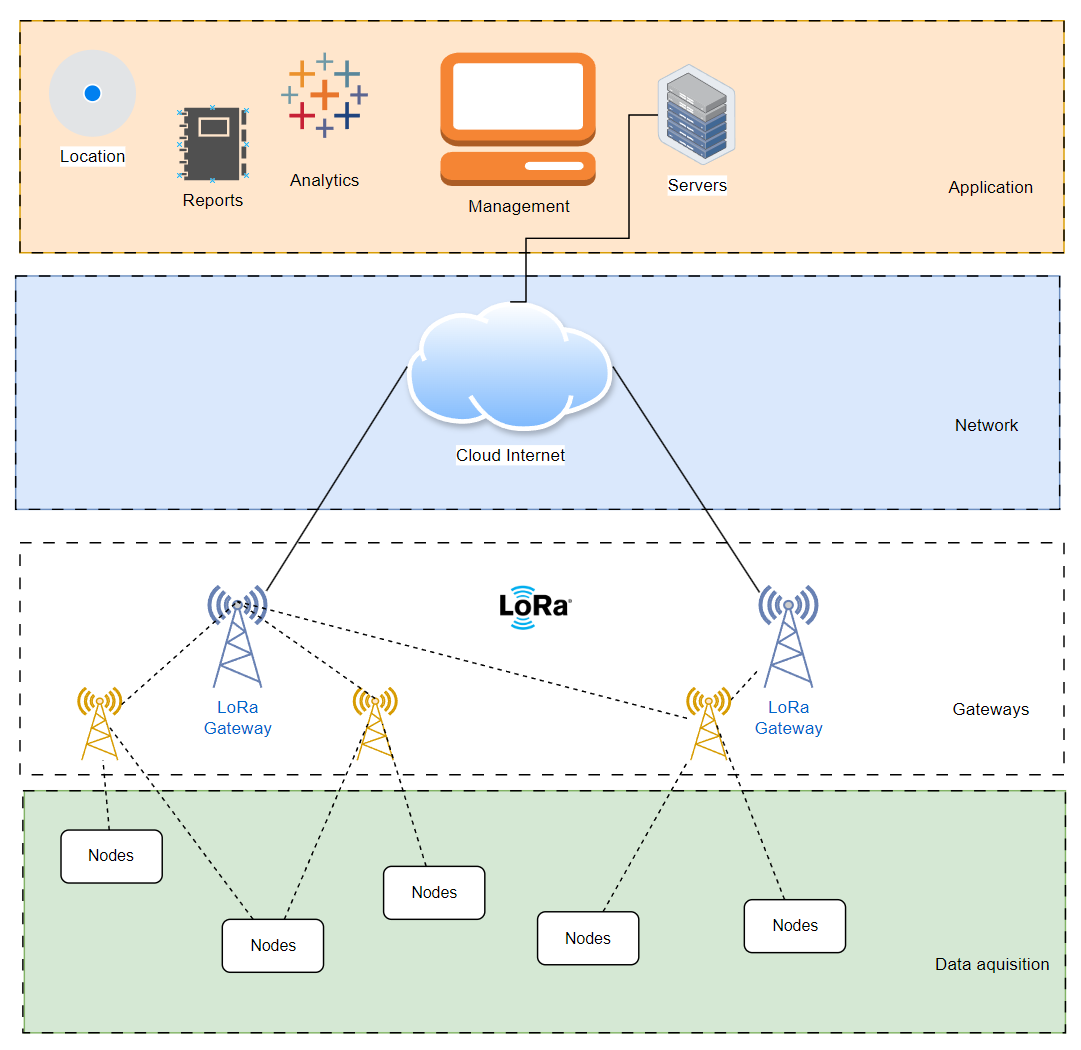
\includegraphics[width=0.7\textwidth]{images/loraWan.png}
    \caption{LoRa-based IoT Architecture for Agriculture}
    \label{fig:lora_architecture}
\end{figure}

\section{LoRa vs Other Wireless Technologies}
At this moment, theere are several wireless technologies available for IoT applications. After a 
comparative analysis of the most popular wireless technologies used in IoT, LoRa came out as one of the most suitable
technologies for smart irrigation systems because of its long range, low power consumption and scalability.
The table below compares LoRa with other wireless technologies commonly used in IoT applications, such as Wi-Fi, Bluetooth (BLE), 
Zigbee, and NB-IoT. In this section We will analyze the capabilities of these technologies
and their suitability for smart irrigation systems. The comparison is based on several features, 
including range, data rate, power consumption, topology, license band, scalability, cloud integration, infrastructure cost and latency.

Wifi, Bluetooth and Zigbee have a decent data rate, and very good latency, but they have a very short range 
and high power consumption. This makes them more suitable for local applications, 
such as home automation or local sensor networks. 
NB-IoT(Narrowband IoT) represents a poteantial solution for smart irrigation systems, but 
it has a higher infrastructure cost and requires a cellular network, which may not be available in all areas.

\begin{table}[ht]
\centering
\begin{tabular}{|p{3.2cm}|p{2.6cm}|p{2.6cm}|p{2.6cm}|p{2.6cm}|p{2.6cm}|}
\hline
\textbf{Feature} & \textbf{LoRa} & \textbf{Wi-Fi} & \textbf{Bluetooth (BLE)} & \textbf{Zigbee} & \textbf{NB-IoT} \\
\hline
Range & 2–15 km & $\sim$100 m & 10–100 m & 10–100 m & 10–35 km \\
\hline
Data Rate & 0.3–50 kbps & Up to 600 Mbps & Up to 2 Mbps & 20–250 kbps & Up to 250 kbps \\
\hline
Power Consumption & Very Low & High & Very Low & Low & Low \\
\hline
Topology & Star (LoRaWAN) & Star & Star & Mesh & Star (cellular) \\
\hline
License Band & Unlicensed (ISM) & Unlicensed (2.4 GHz) & Unlicensed (2.4 GHz) & Unlicensed (2.4 GHz) & Licensed \\
\hline
Scalability & High & Low & Low–Medium & Medium & High \\
\hline
Cloud Integration & Easy via LoRaWAN & Native IP stack & Requires gateway & Requires gateway & Native via operator \\
\hline
Infrastructure Cost & Low & Medium & Low & Medium & High \\
\hline
Latency & High (seconds) & Low (ms) & Very Low (ms) & Low (ms) & Moderate \\
\hline
Ideal Use Case & Smart City Infrastructure & Local, high-speed data transfer & Short-range sensors/wearables & Indoor sensor networks & National-scale deployment \\
\hline
\end{tabular}
\caption{Comparison of Wireless Technologies for Smart Irrigation}
\label{tab:wireless_comparison}
\end{table}


\section{Identified Gaps and Challenges}
Despite the advancements in smart irrigation systems, several gaps and challenges remain:

\begin{itemize}
  \item \textbf{High Costs} \\
  Many existing systems are expensive, making them inaccessible for small farmers or home gardeners.
  
  \item \textbf{Complexity of Use} \\
  Some systems require specialized knowledge to set up and maintain, which can be a barrier for adoption.

  \item \textbf{Limited Customization} \\
  Many commercial solution are designed for speicific crops and environments and that limits their
  applicability to diverse agricultural settings.
  \item \textbf{Data Integration Issues} \\
  Integration of data from different sources (e.g. wather, soil) can be more 
  complex and it can lead to inefficiencies in the irrigaiton management.
\end{itemize}

In addition to the gaps mentioned, there are a few other issues that must be resolved, 
like the need for systems that can function in challenging environmental conditions, 
the need for dependable internet connectivity in remote locations, and data security and privacy issues. 

The effect that smart irrigation systems have on the environment is another factor that must be 
taken into account.
Even though these systems are made to use water as efficiently as possible, the manufacturing 
and disposal of electronic components can harm the environment.
Therefore, developing sustainable and ecologically friendly systems is another challenge. 
This means that the systems should be built to last a long time and be simple to use, 
and that the parts used in them should be composed of recyclable materials.

\section{Summary}
In summary, the state of the art in smart irrigation systems shows significant 
advancements in technology and methods, but also highlights several gaps and challenges 
that need to be addressed. The PiIrrigate project aims to fill these gaps by providing a
cost-effective, easy-to-use, and customizable solution that leverages the power of IoT and LoRa 
\chapter{Used Technologies}
\section{Development Process Tools}
\subsection{Version Control: GitHub}
GitHub is a web-based platform that uses Git for version control and collaboration on software projects.
It enables developers to collaborate in real-time. Thhey can track changes, manage issues, and review code.
It was released in 2008 and in 2018 it was acquired by Microsoft\cite{githubDefinition}.
Github is widely used in the software development industry and in has become standard practice to 
use GitHub for version control. 

\subsection{Software Development: Visual Studio Code and Visual Studio}
Visual Studio Code (VS Code) is a free lightweight code editor developed by Microsoft.
It supports a wide range of programming langueges and has a rich collection of extensiont that can be used to 
enchance its functionality\cite{vscode}.
It was very convinient to use a single code editor for multiple programming languages and frameworks.
To be more specific, I used Visual Studio Code for ESP32 programming, along with Platform IO, 
which is an open-source ecosystem for IoT development. VSCode was also used for the Angular web application 
development. The Raspberry Pi was programmed using Python, I used Visual Studio Code and for remote access
I used SSH.

Visual Studio is a more comprehensive integrated development environment (IDE) that provides advance features
for software development, such as debugging, profiling, and testing.
Visual Studio is also developed by Microsoft and it is widely used in the software development industry.
Since the PiIrrigate's web API was developed in .NET, I used Visual Studio for the API development\cite{vs}.

\subsection{System Architecture: Draw.io}
Draw.io is a free online diagramming tool that allows users to create flowcharts, 
UML diagrams, network diagrams, and more. 
Other alternatives include Lucidchart, Microsoft Visio, and Gliffy. But I found that Draw.io is easy to use
and provides a wide range of templates and shapes that can be used to create diagrams\cite{drawio}.

\subsection{Iot Device Management: Azure IoT Hub}
Azure IoT Hub is a managed service service that acts as a central message hub in a cloud-based IoT solution. It enables reliable and secure
communication at a scale between an IoT application and its attached devices. Almost any device can be connected to an IoT hub\cite{Iothub}.
Azure IoT Hub is used in the PiIrrigate project to manage the
communication between the Raspberry Pi and the web API.

\section{Communication Technologies}
\subsection{LoRa Radio Communication}
LoRa is a wireless modulation technique derived from Chirp Spread Spectrum (CSS) technology.
LoRa modulated transmission is robust against disturbances and can be received across great distances.
It has become popular, as one of the most used standards for device interconnection, mainly because of its
low power consumption and long-range capabilities\cite{lora}. This technology was used in the PiIrrigate project
to enable the communication between the ESP32 nodes and the ESP32 gateway connected to the Raspberry Pi.

\subsection{MQTT Protocol}
MQTT (Message Queuing Telemetry Transport) is a 
an OASIS standard lightweight messaging protocol for the Internet of Things (IoT).
It is designed as an extremely lightweight publish/subscribe messaging transport that is ideal for connecting 
remote devices with a small code footprint and minimal network bandwidth. 
In the PiIrrigate project, MQTT is used to send data from the Raspberry Pi to IoTHub
and from the web API to the web application\cite{mqtt}.

\subsection{HTTP Protocol}
HTTP is an application layer protocol for transmitting hypermedia documents, such as HTML.
It was designed for communication between web browsers and servers, 
but it can also be used for machine-to-machine communication.
In the PiIrrigate project, HTTP is used to send data from the web API to the web application\cite{http}.

\subsection{SignalR and WebSockets}
SignalR is an open-source library for ASP.NET that simplifies 
the process of adding real-time web functionality to applications.
It allows server-side code to push content to connected clients instantly as it becomes available.
SignalR uses WebSockets as its primary transport protocol, but it can also fall back to other techniques like
Server-Sent Events or Long Polling if WebSockets are not available\cite{signalrandwebsockets}.
In the PiIrrigate project, SignalR is used to provide real-time communication 
between the web API and the web application.

\section{Programming Languages and Frameworks}
\subsection{C\# and .NET}
C\# is a modern, object-oriented programming language developed by Microsoft.
It is widely used for developing Windows applications, web applications, and cloud services.
.NET is a free, open-source developer platform that provides a wide range of tools and libraries 
for building applications \cite{csharp}.
In the PiIrrigate project, C\# and .NET are used to develop the web API that manages the communication
between the Raspberry Pi and the web application, as well as to handle data storage in the PostgreSQL database
\cite{dotnet}.

\subsection{Entity Framework Core}
Entity Framework Core (EF Core) is an open-source, lightweight, extensible, and cross-platform version 
of the Entity Framework, which is an object-relational mapper (ORM) for .NET.
EF Core allows developers to work with databases using .NET objects, eliminating the need for 
most of the data access code that developers usually need to write\cite{efcore}.
In the PiIrrigate project, EF Core is used to interact with the PostgreSQL database.

\subsection{Python}
Python is a high-level, interpreted programming language known for its simplicity and readability.
It is widely used in various domains, including web development, data analysis, machine learning, and IoT\cite{python}.
In the PiIrrigate project, Python is used to develop the code that runs on the Raspberry Pi,
which is responsible for receiving data from the ESP32 nodes and sending it to the web API.

\subsection{Arduino C/C++}
Arduino C/C++ is a simplified version of C/C++ that is used to program Arduino 
boards and other microcontrollers\cite{arduino}.
It provides a set of libraries and functions that make it easy to interact with hardware components.
In the PiIrrigate project, Arduino C/C++ is used to program the ESP32 nodes that collect data from the sensors
and send it to the gateway using LoRa radio communication.

\subsection{Angular and TypeScript}
Angular is a platform and framework for building single-page client applications using HTML and TypeScript.
It is developed and maintained by Google and is widely used for building modern web applications\cite{angular}.
In the PiIrrigate project, Angular is used to develop the web application that provides a user interface for
monitoring and controlling the irrigation system.

TypeScript is a superset of JavaScript that adds static typing and other features to the language.
It is designed for large-scale applications and provides better tooling and error checking compared to JavaScript.
JavaScript is a high-level, interpreted programming language that is widely used for building web applications.
It is primarly used for client-side scripting, but it can also be used for
 server-side development using Node.js\cite{typescript}.

\chapter{PiIrrigate System Overview}\label{section:overview}

\section{Overview}
The Internet of Things (IoT) is a new technology that allows devices to connect remotely to achieve smart
farming \cite{agriculture12101745}. The IoT has a wide range of applications in agriculture, and it has 
began to influence many other industries as well, such as healthcare, transportation, and manufacturing. 
This was done to improve the efficiency and productivity of these industries, 
as well as to reduce costs and improve the quality of products and services\cite{s19081833}.

The PiIrrigate smart irrigation system is build using a combination of hardware and software technologies.
It leverages both low-power edge devices and cloud-based infrastructure to provide real-time monitoring
and data collection, as well as remote control capabilities.
The core components and their roles in the system are as follows:
\begin{itemize}
  \item \textbf{ESP32 (LILYGO Meshtastic AXP2101 T-Beam V1.2 ESP32 LoRa)} \\
  The LILYGO Meshtastic AXP2101 T-Beam V1.2 ESP32 LoRa is a development board based on the ESP32 microcontroller, it is equipped with
  LoRa radio communication capabilities, Wifi, Bluetooth, GPS, and a battery management system.
  It is used to collect data from sensors and send it to the gateway using LoRa radio communication.

  \item \textbf{Raspberry Pi} \\
  Raspberry Pi is a small, affordable computer that can be used for a wide range of applications.
  The Raspberry Pi is the core of the PiIrrigate irrigation module, 
  it is responsible for receiving data from the ESP32 nodes and sending it to Azure IoT Hub.

  \item \textbf{Azure IoT Hub} \\
  Azure IoT Hub is a cloud-based service that enables secure and reliable communication 
  between IoT devices and the cloud.
  It manages the bidirectional communication between the Raspberry Pi and the web API.

  \item \textbf{Web API} \\
  The web API is developed in .NET and is responsible for receiving data from the Raspberry Pi,
  storing it in a PostgreSQL database, and providing a way to access the data.
  SignalR is used to provide real-time communication between the server and the client.
  It also provides a way to control the system manually and to add new nodes to the system.

  \item \textbf{PostgreSQL Database} \\
  PostgreSQL is a powerful, open-source relational database management system.
  It is used to store the data collected from the sensors and the schedules sent to the system. It also
  stores the user data and the configuration of the system. The database is hosted in Neon.

  \item \textbf{Web Application} \\
  The web applicaiton is developed using Angular and is responsible for displaying live, historical data
  and provide the user interface for controlling the system.
\end{itemize}

In the following sections, we will explore each of these components in more detail,
starting with the hardware components and then moving on to the software components.

\section{Hardware Components}
\subsection{Sensors}
The PiIrrigate system uses a variety of sensors to collect data from the environment.
The sensors used in the PiIrrigate system are:
\begin{itemize}
  \item \textbf{Soil Moisture Sensor} \\
  The soil moisture sensor is used to measure the moisture level in the soil. It is used to determine when to irrigate the plants.
  The sensor is connected to the ESP32 board and sends the data to the gateway using LoRa radio communication.

  \item \textbf{Temperature and Humidity Sensor} \\
  The temperature and humidity sensor is used to measure the temperature and humidity of the environment.
  It is used to determine the optimal conditions for plant growth and to adjust the irrigation schedule accordingly.

  \item \textbf{Rain Sensor} \\
  The rain sensor is used to detect rain and prevent irrigation during rainy weather. 
  It helps to conserve water and prevent over-irrigation.

  \item \textbf{Water Flow Sensor} \\
  The water flow sensor is used to measure the flow rate of water in the irrigation system.
  It is used to monitor the water consumption.

  \item \textbf{Water Temperature Sensor} \\
  The water temperature sensor is used to measure the temperature of the water in the irrigation system.
  It is used to ensure that the water temperature is within the optimal range for plant growth.


\end{itemize}
\subsection{ESP32 (LilyGo T-Beam)}

The T-Beam ESP32 LoRa Wireless Module is a compact development board thaht combines an ESP32 microcontroller,
LoRa transceiver (SX1278), GPS module, and a battery management system into a single unit. This board is ideal
for long-range, low-power IoT applications such as mesh networks, asset tracking, smart agriculture and environmental
monitoring. Besides this, it has a built-in OLED display. The communication range of the LoRa transceiver can reach up to 10 km in open areas.
\begin{figure}[H]
    \centering
    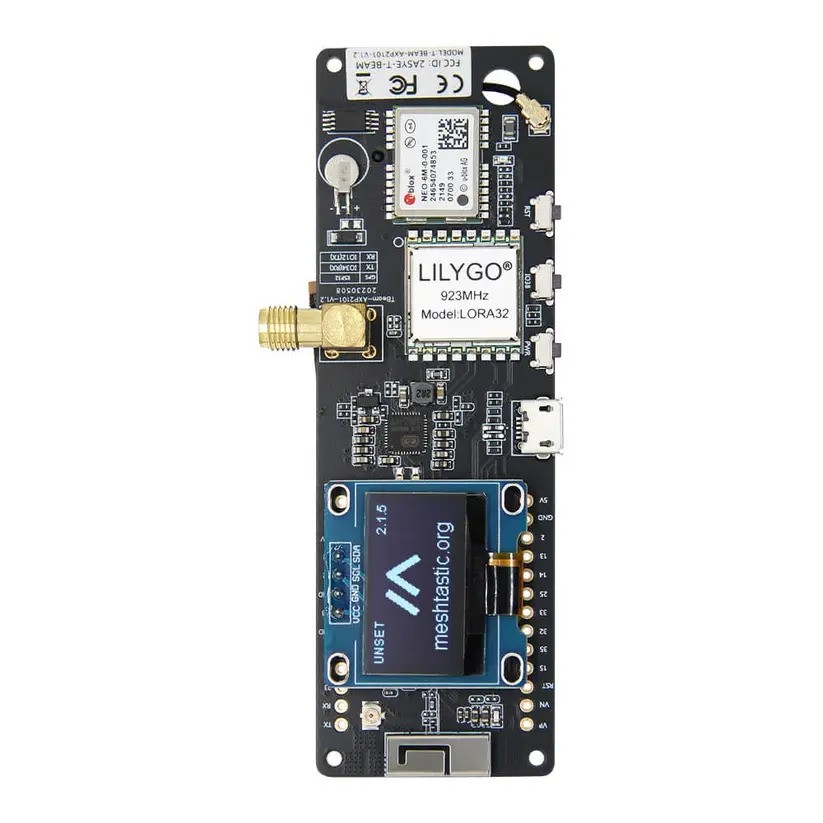
\includegraphics[width=0.8\textwidth]{images/esp32lora.jpg}
    \caption{ESP32 (LilyGo T-Beam) module used in PiIrrigate}
    \label{fig:esp32lora}
\end{figure}

\subsection{Raspberry Pi 4 Model B}
The Raspberry Pi 4 Model B is a small, affordable computer that can be used for a wide range of applications.
It is equipped with a quad-core ARM Cortex-A72 processor, up to 8GB of RAM, and supports dual-band Wi-Fi and Bluetooth.
The Raspberry Pi 4 Model B together with an ESP32LoRa is used in the PiIrrigate project as the gateway that receives data from the ESP32 nodes
and sends it to IoT Hub.
\begin{figure}[H]
    \centering
    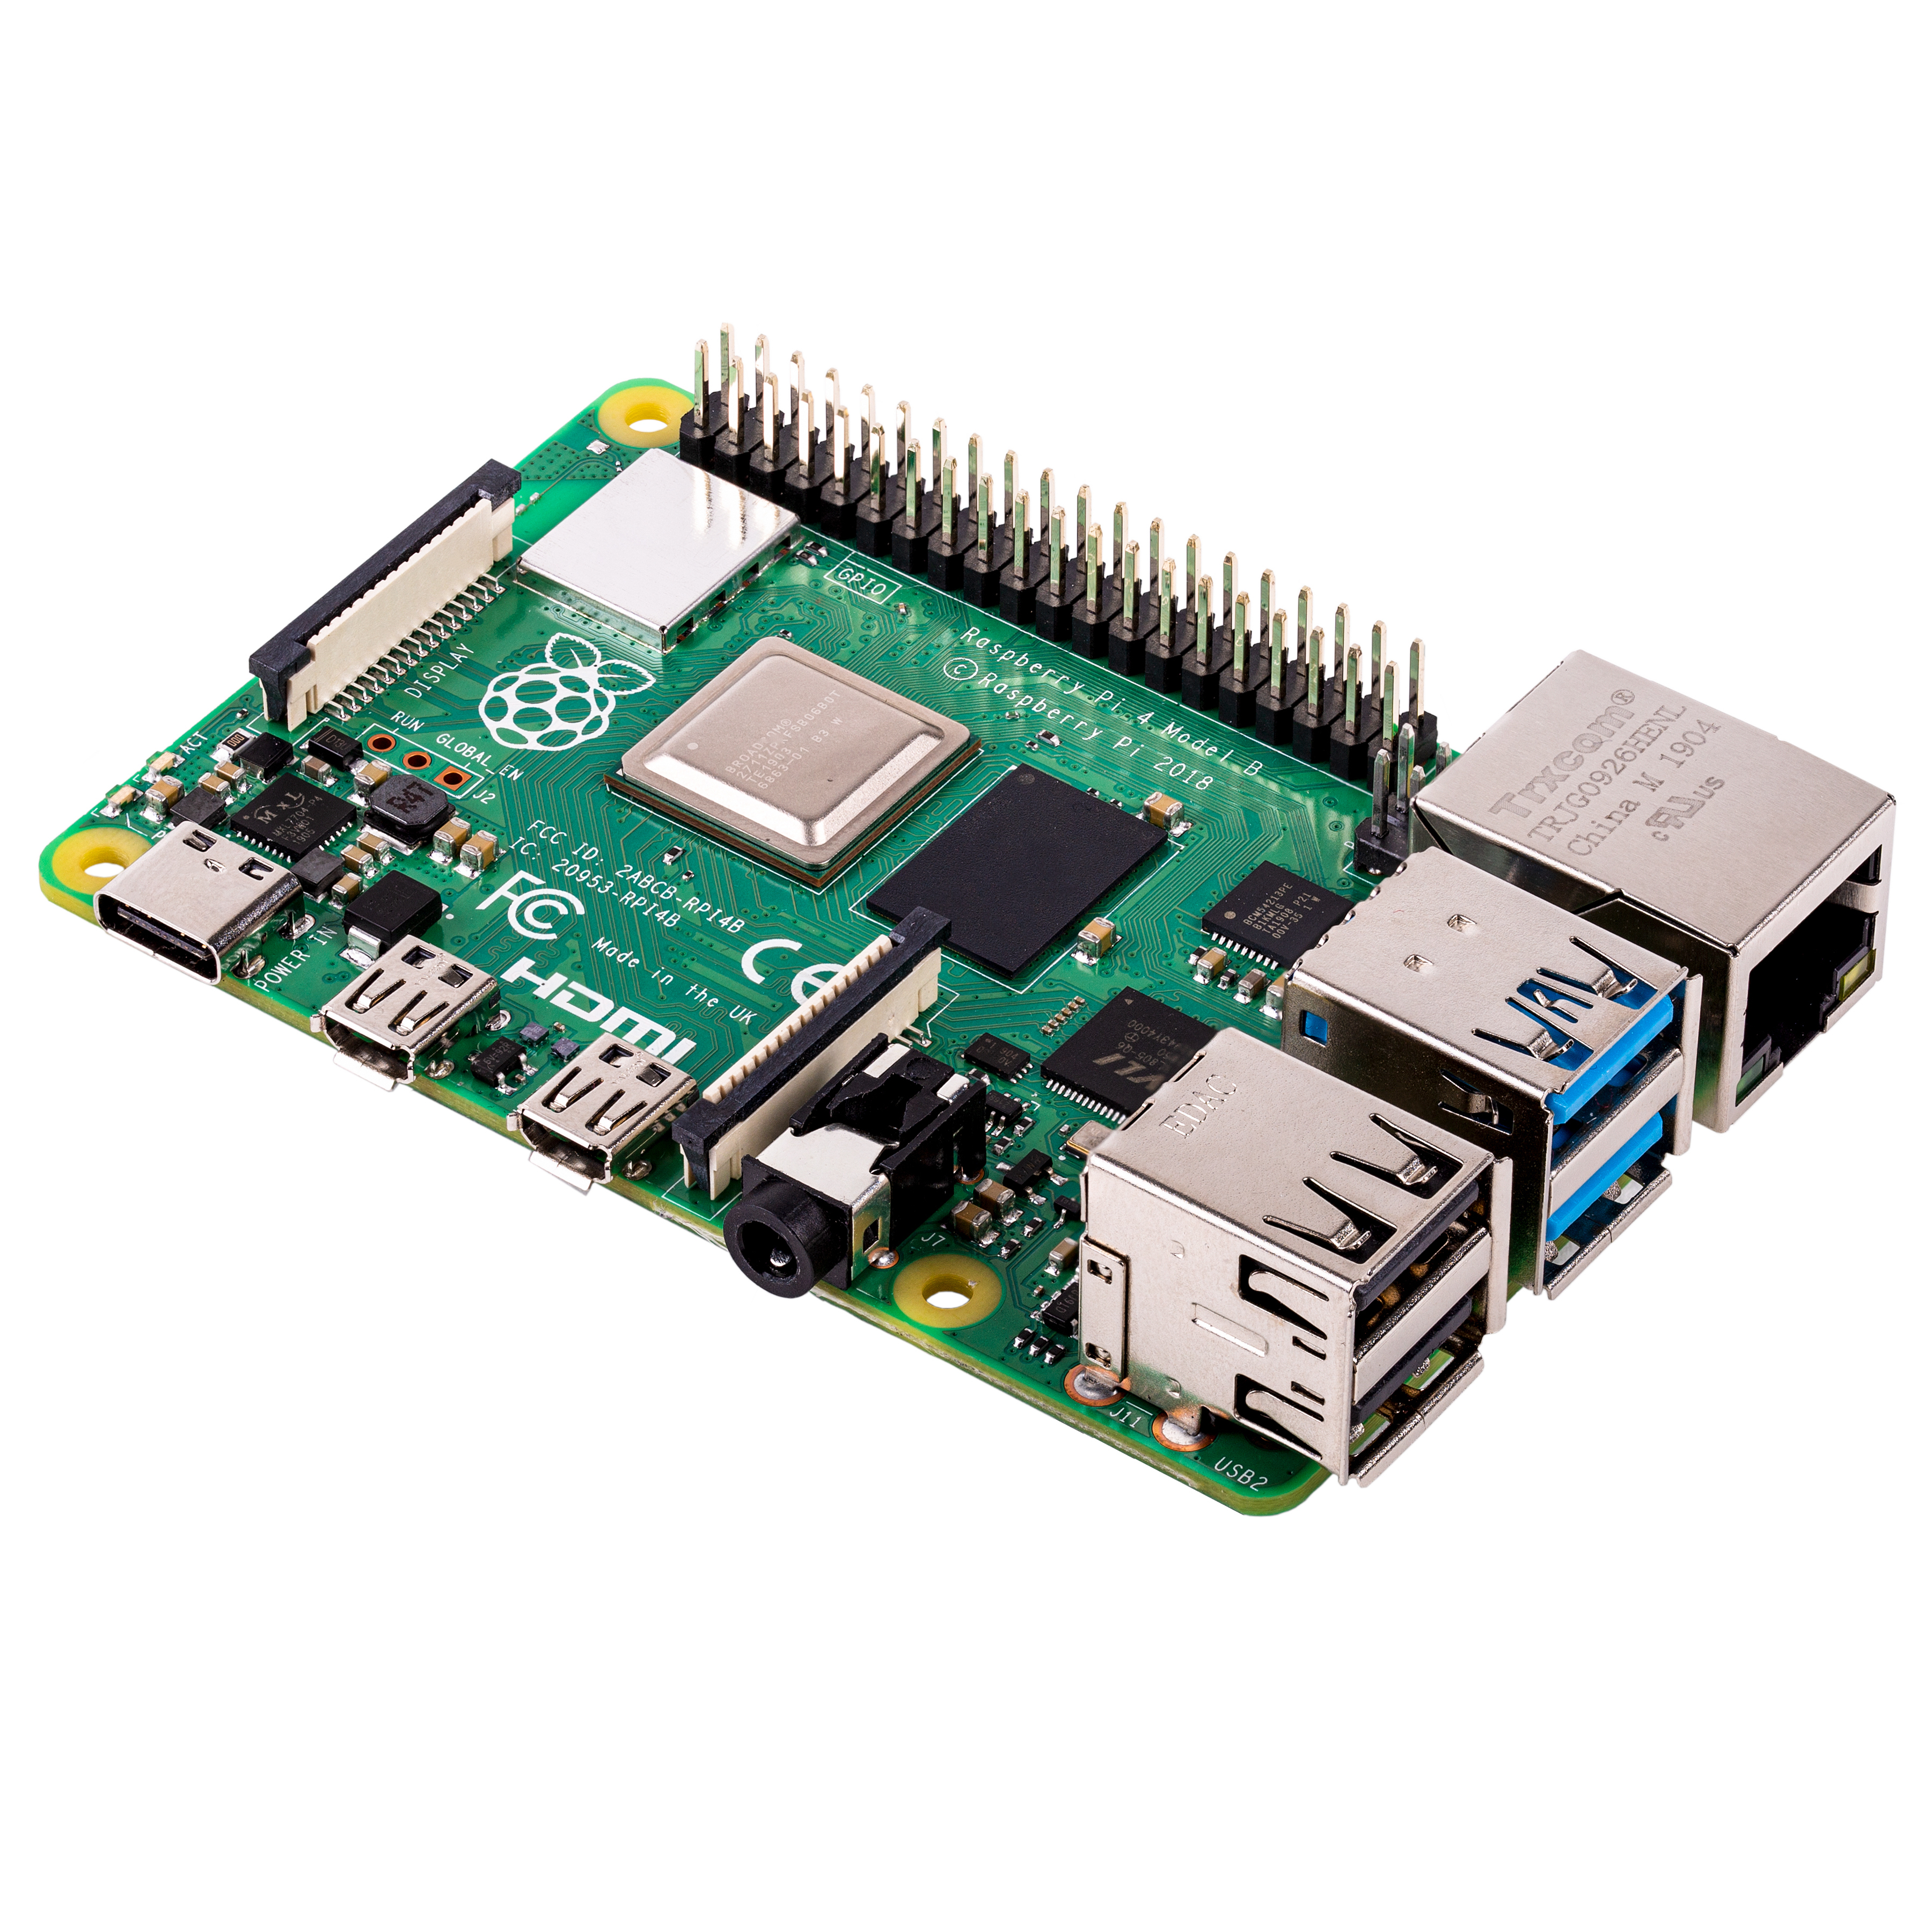
\includegraphics[width=0.8\textwidth]{images/raspberrypi.jpg}
    \caption{Raspberry Pi 4 Model B used in PiIrrigate}
    \label{fig:raspberrypi}
\end{figure}

\section{Hardware Architecture}
The hardware architecture of the PiIrrigate system consists 
of multiple ESP32 nodes that collect data from the sensors and send it to a gateway ESP32 connected to a Raspberry Pi.
The Raspberry Pi acts as a gateway that receives data from the ESP32 nodes and sends it to Azure IoT Hub using MQTT protocol.
The ESP32 nodes are connected to various sensors that collect data from the environment.

The ESP32 nodes are connected to the sensors and actuators as follows:
\begin{itemize}
  \item Soil moisture (YL-69) sensor is connected to GPIO32.
  \item Temperature and humidity sensor (DHT11) is connected to GPIO27.
  \item Rain sensor (YL-83) is connected to GPIO32.
  \item Water flow sensor {YF-S201} is connected to GPIO35.
  \item Water temperature sensor (DS18B20) is connected to GPIO26.
  \item The relay module that controls the electronic valve is connected to GPIO22.
\end{itemize}

In the figure below, you can see a simplified digram of the ESP32 pinout and connections.

\begin{figure}[H]
    \centering
    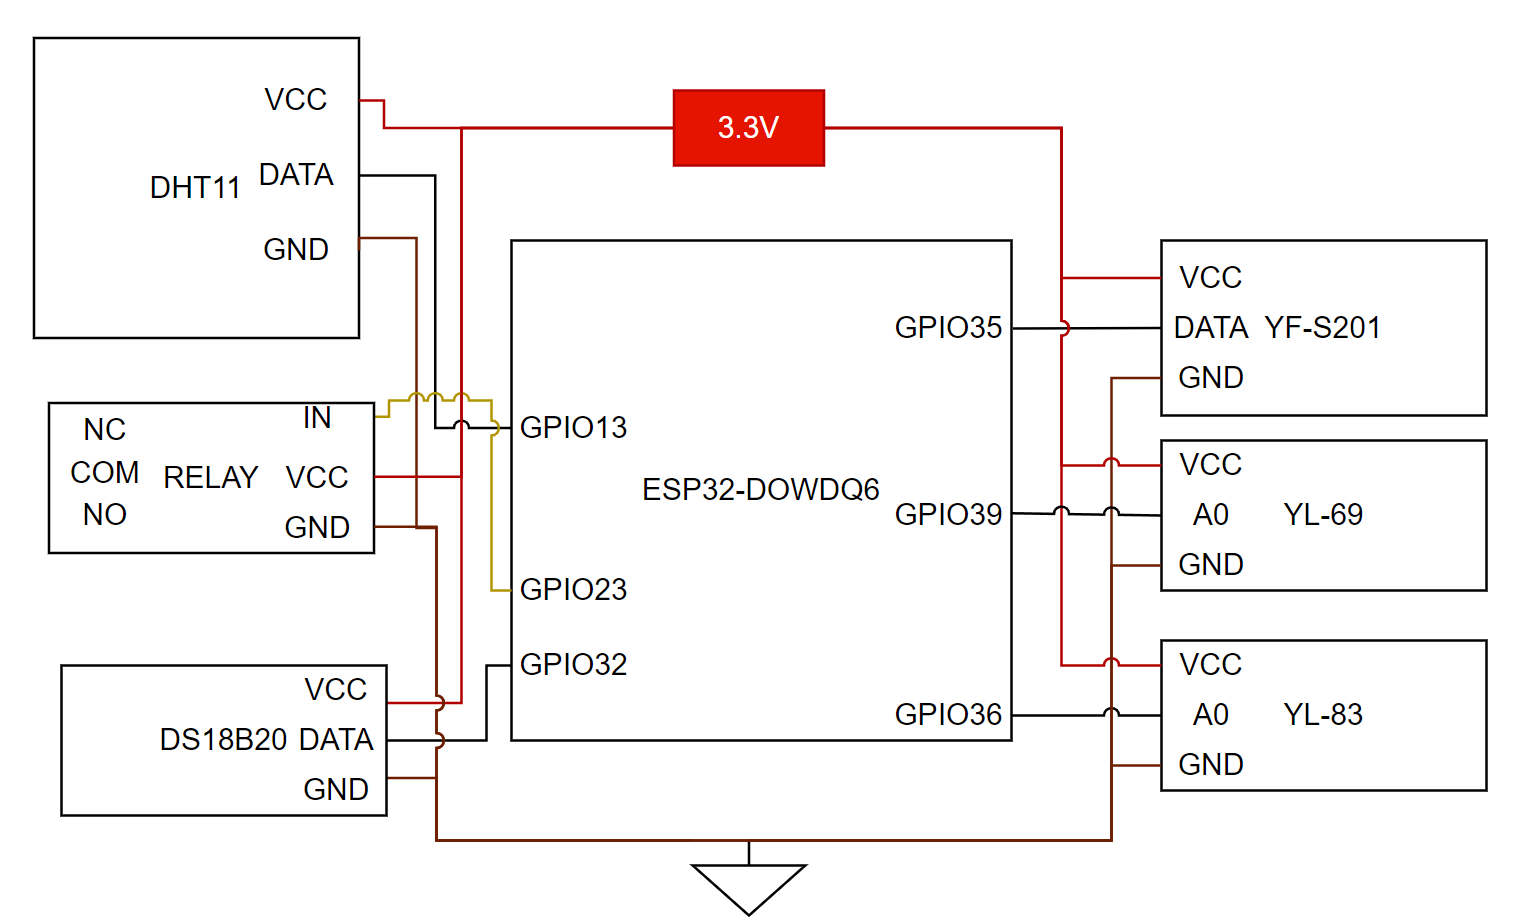
\includegraphics[width=0.8\textwidth]{images/esp-diagram.png}
    \caption{ESP32 pinout and connections}
    \label{fig:esp32-pinout}
\end{figure}

The communication between the gateway ESP32 and the Raspberry Pi is done using UART (Universal Asynchronous Receiver-Transmitter) protocol.
The gateway ESP32 receives data from the nodes using LoRa radio communication and sends it to the Raspberry Pi using UART.
In the figure below it is described the connection between the ESP32 and the Raspberry Pi.

\begin{figure}[H]
    \centering
    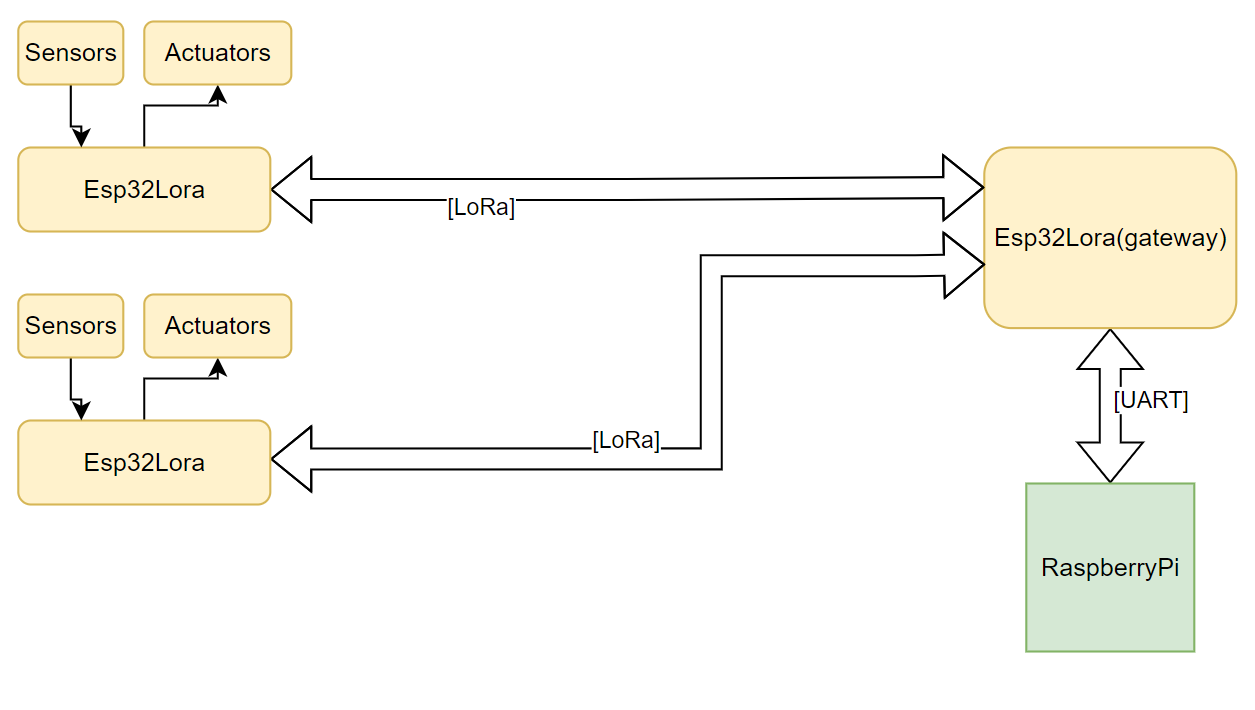
\includegraphics[width=0.8\textwidth]{images/hardware-architecture.png}
    \caption{ESP32 Gateway connection to Raspberry Pi}
    \label{fig:esp32-gateway}
\end{figure}

\section{Data Flow}
The data flow in the PiIrrigate system is as follows:

\begin{enumerate}
  \item The ESP32 nodes collect data from the sensors and send it to the gateway using LoRa radio communication.
  \item The Raspberry Pi receives the data from the ESP32 nodes and sends it to Azure IoT Hub using MQTT protocol.
  \item The web API receives the data from Azure IoT Hub and stores it in the PostgreSQL database using Entity Framework Core. 
  \item The web application retrieves the data from the web API and displays it to the user in real-time using SignalR.
\end{enumerate}
\begin{figure}[H]
    \centering
    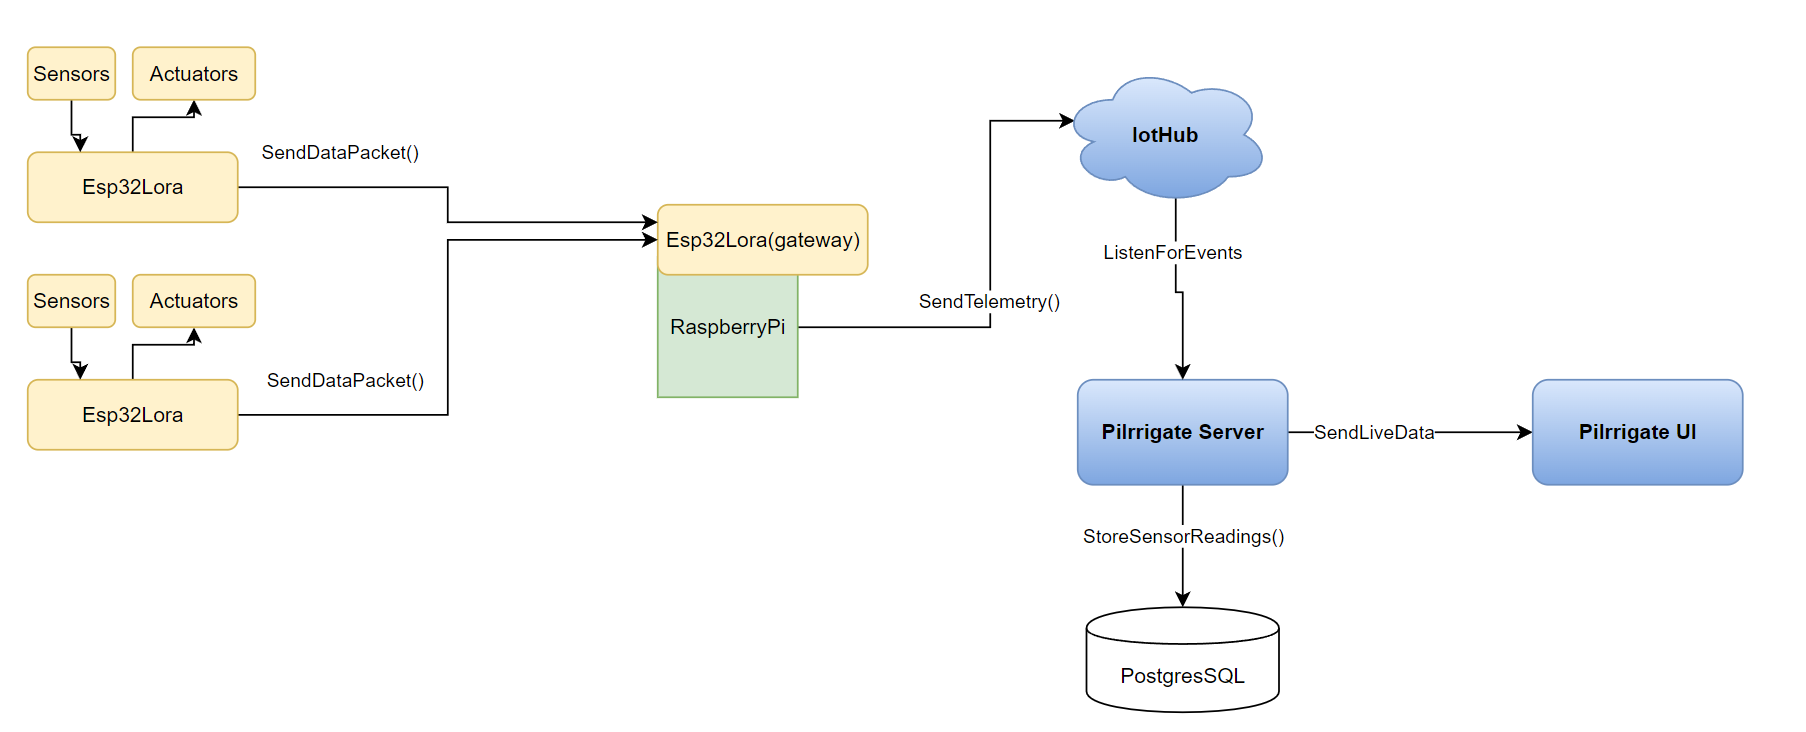
\includegraphics[width=0.8\textwidth]{images/system.png}
    \caption{PiIrrigate System overview}
    \label{fig:system-overview}
\end{figure}

\subsection{Data aquisition}
The data acquisition is done using the ESP32 nodes that collect data from the sensors.
For each sensor type, I created a specific library thath can be used to read the data from the sensor.
Temperature and humidity data is collected using a DHT11 sensor. The communication with the sensor is done using
1-wire digital interface. The communication is done in 3 steps\cite{1wire}:
\begin{enumerate}
  \item The microcontroller initiates communication by sending the start signal.
  The start signal is an 18\,ms LOW signal followed by a $20$--$40\,\mu$s HIGH signal.
  \item The sensor responds a fixed LOW and HIGH handshake pattern, indicating that it is ready to send data.
  Usually the acknowledgment is a $80\,\mu$s LOW signal followed by a $80\,\mu$s HIGH signal.
  \item After the handshake, the sensor sends a 40-bit data stream, which includes the humidity and temperature data.
  The bits are sent in a specific order: first the humidity data (16 bits), 
  then the temperature data (16 bits), 
  and finally a checksum (8 bits).
  Each bit is sent as a $50\,\mu$s LOW signal followed by a HIGH signal that lasts for either $26$--$28\,\mu$s (for a 0 bit) or $70\,\mu$s (for a 1 bit).
  In code, for each bit, the microcontroller waits for the LOW signal to start, 
  then waits for $30\,\mu$s then ig the signal is HIGH, the bit is a 1, otherwise it is a 0.
  The checksum is used to verify the integrity of the data received from the sensor.
\end{enumerate}

\begin{figure}[H]
    \centering
    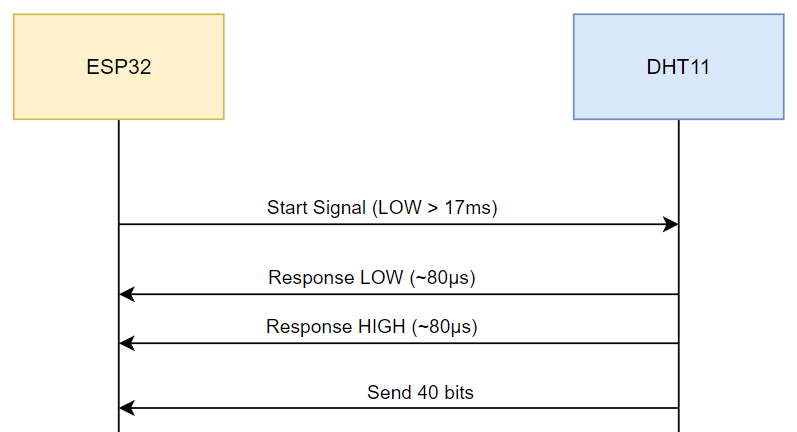
\includegraphics[width=0.8\textwidth]{images/dht-steps.png}
    \caption{Steps in data aquisition from DHT11 sensor}
    \label{fig:dht-steps}
\end{figure}

For the soil moisure data acquisition, I used a resistive soil moisture sensor. The principle of operation is based
on measuring the resistance of the soil. The sensor consists of two probes that are inserted into the soil.
When the soil is dry, the resistance between the probes is high, and when the soil is wet, the resistance is low\cite{s20020363}.
Then an ADC is used to measure the voltage across the probes, which is transofmerd into digital value. In this case, the
ADC is a 12-bit ADC, which means that the digital value can range from 0 to 4095.

For the rain sensor, I used a resistive rians sensor. The principle of operation is similar to the soil moisture sensor,
but it is designed to detect the presence of water on the sensor surface. 
When the sensor is dry, the resistance between the probes is high, and when it is wet, the resistance is low.

\begin{figure}[H]
    \centering
    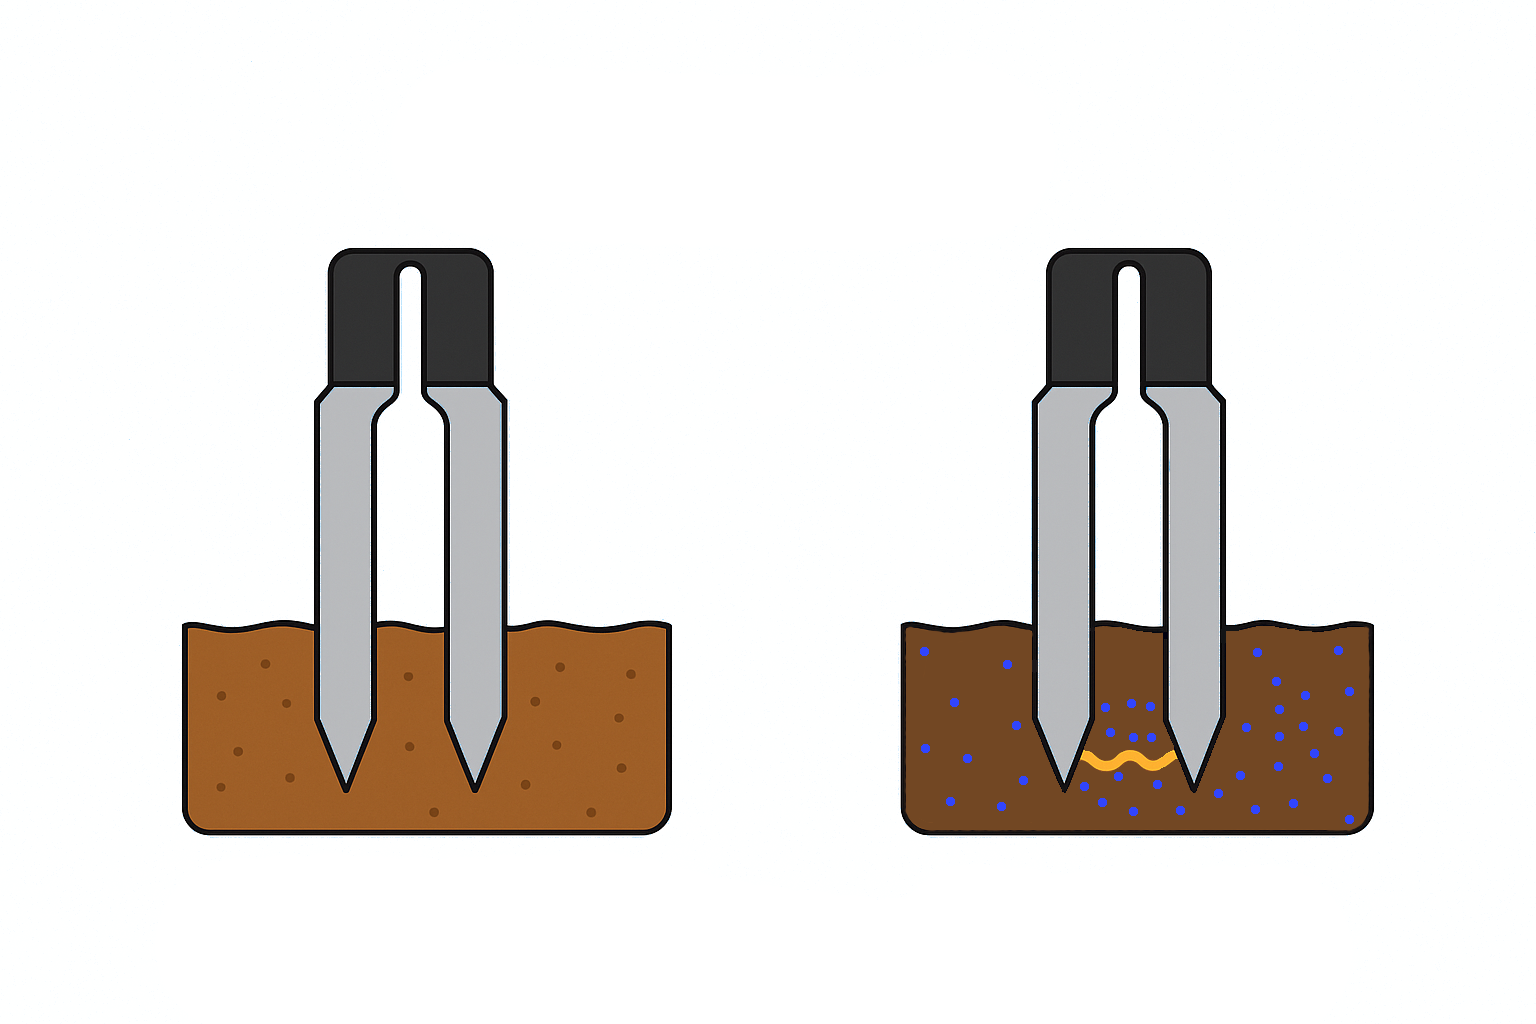
\includegraphics[width=0.7\textwidth]{images/moisture-sensor.png}
    \caption{Soil moisture sensor based on resistive principle}
    \label{fig:moisture-sensor}
\end{figure}

Since the water consumoption is a very important aspect in agriculture, 
I wanted to add a water flow sensor to the system. For the purpose of this project I used an 
YF-S201 water flow sensor, 
which is a low-cost sensor that can be used to measure the flow rate of water in a pipe.
The sensor consists of a plastic body with a 
turbine inside that rotates when water flows through it.
The rotation of the turbine generates a pulse signal that can be used to measure the 
flow rate of water.
The sensor has a maximum flow rate of 30 liters per minute and a minimum 
flow rate of 1 liter per minute.
The sensor has three wires: red (VCC), black (GND), and yellow (signal).
At each rotation of the tubine, the sesnsor generates a pulse signal on the signal wire.
The ESP32 counts the number of pulses in a given time interval 
(e.g., 1 second) to calculate the flow rate.
The flow rate can be calculated using the following formula:
\begin{equation}
    \text{Flow Rate} = \frac{\text{Number of Pulses} \times 60}{\text{Time Interval (seconds)}}
\end{equation}
\begin{figure}[H]
    \centering
    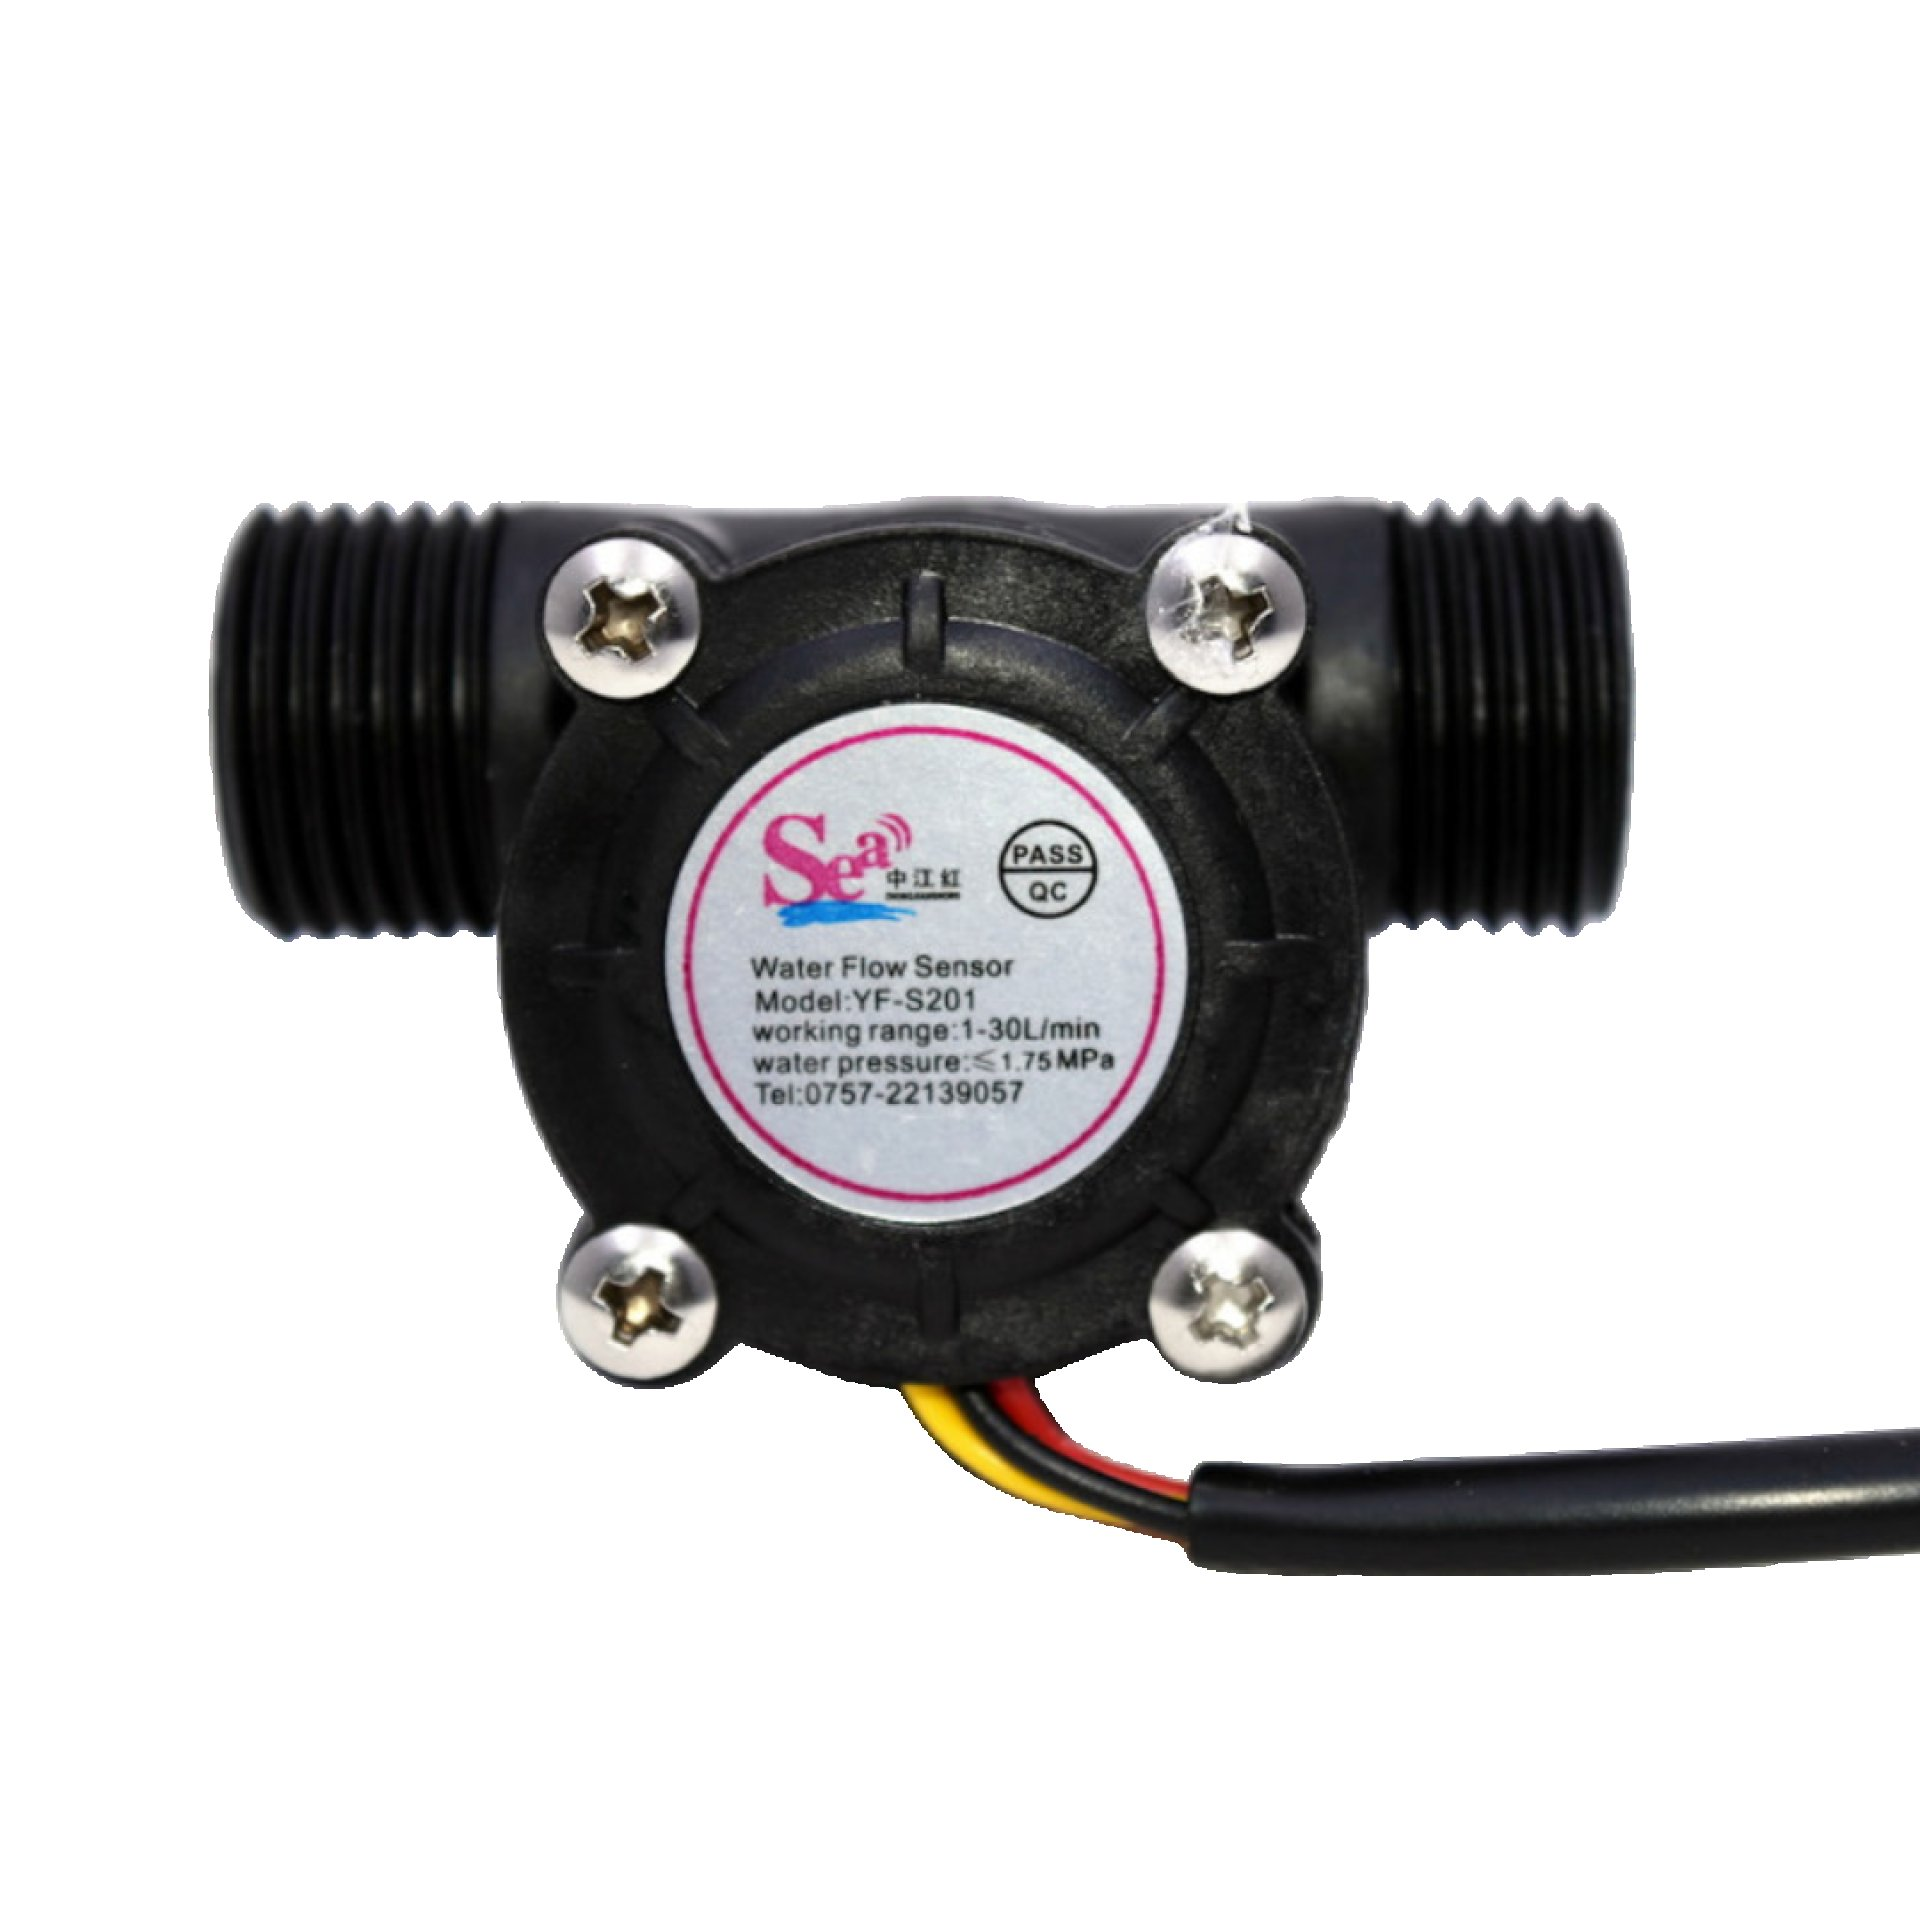
\includegraphics[width=0.5\textwidth]{images/water-flow.jpg}
    \caption{Water flow sensor used in PiIrrigate}
    \label{fig:water-flow-sensor}
\end{figure}

In my implementation, the water will be in a container, and during the irrigation process, 
the water will be deliverd to the plants using the gravity force. Because of this, I used
water temperature sensor to measure the temperature of the water in the container. 
The water temperature sensor is a DS18B20 sensor, 
which is a digital temperature sensor that can be used to measure the temperature of liquids.
The DS18B20 sensor uses the 1-wire digital interface to communicate with the ESP32.
The sensor can measure temperatures from -55°C to +125°C with an accuracy of ±0.5°C.

\begin{figure}[H]
    \centering
    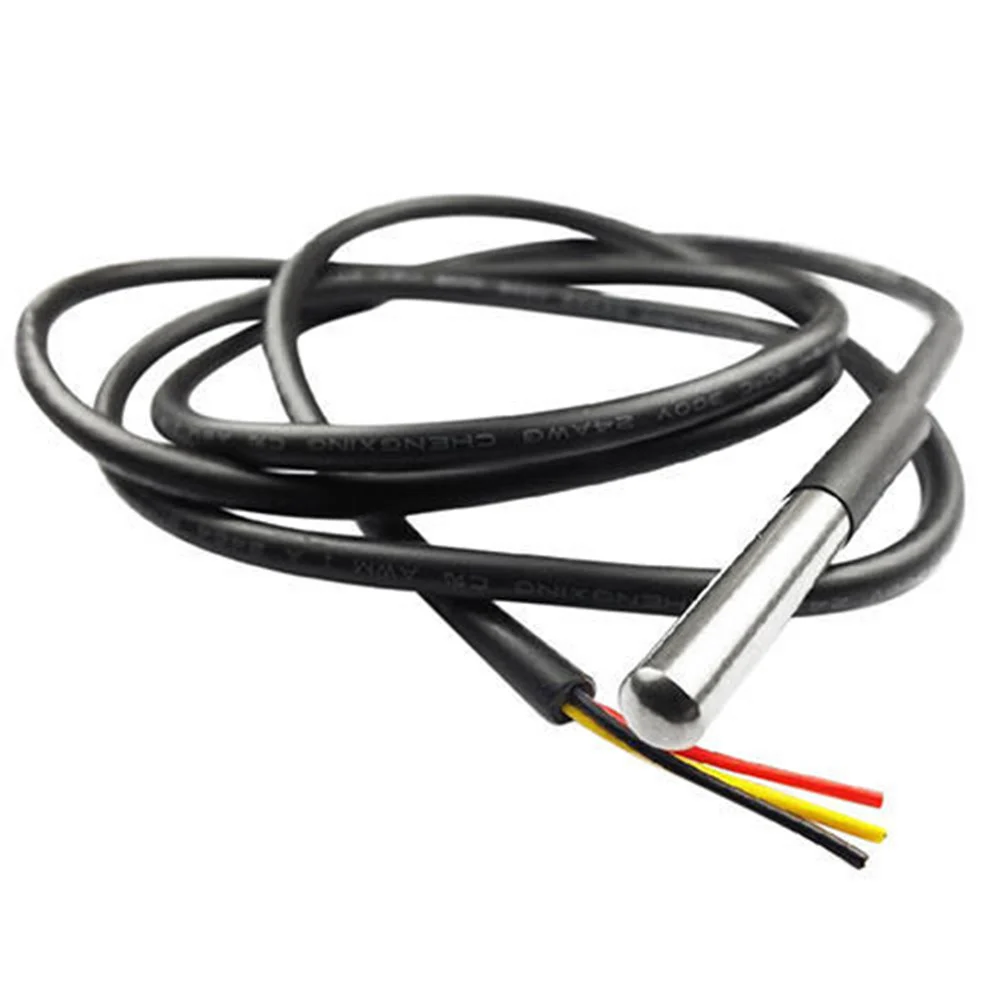
\includegraphics[width=0.5\textwidth]{images/water-temp.png}
    \caption{DS18B20 water temperature sensor used in PiIrrigate}
    \label{fig:ds18b20}
\end{figure}

Beside the sensors, I also used the GPS module of the T-Beam ESP32 board to 
ollect the GPS coordinates of the node. 
This can be useful for tracking the location of the node and for mapping the irrigation system.
The LILYGO Meshtastic AXP2101 T-Beam V1.2 ESP32 LoRa development board has a
NEO-6M GPS module, which is a high-performance GPS module that can provide accurate location data.

The GPIO25 pin of the ESP32 board is used to control the relay module that controls 
the electronic valve that opens and closes the water flow to the plants.
The relay module is a simple electronic switch that 
can be used to control high-voltage devices, such as water pumps or valves.

\subsection{LoRa Radio Communication}
LoRa (Long Range) is a wireless communication technology 
that is designed for long-range, low-power applications.
In this implementation, LoRa is used to send data from the nodes to the gateway.
The sensor reading has a period of 10 seconds, which is the default value, but this can be changed from the Web Application.
The data collected from the sensors is serialized into a sensor reading structure, 
which is then is included in a LoRa packet structure that will be 
binary serialized and sent over LoRa radio communication.

\begin{lstlisting}[language=C, caption={LoRa packet structure}]
struct LoRaPacket {
    int packetCount;      // Packet count for tracking
    SensorData sensorData; // Sensor data to be sent
    int stationMac[6]; // MAC address of the device
};
\end{lstlisting}

\begin{lstlisting}[language=C, caption={Sensor reading structure}]
struct SensorData {
    float temperature;
    float humidity;
    float soilMoisture;
    float rainLevel;
    float waterTemp;
    float totalWaterFlow;
    float longitude;
    float latitude;
};
\end{lstlisting}

All the values, except the totalWaterFlow, and the GPS coordinates, represent the raw
voltage values read from the sensors. I chose to sent the raw values, 
because they can be used to calculate the actual values in the web application.
Allowing a better flexibility in the future.

\subsection{Raspberry Pi and ESP32 Gateway}
The gateway ESP23 act like a proxy between the nodes and the Raspberry Pi.
It receives the LoRa packets from the nodes, and then it sends the data to 
the Raspberry Pi using Serial communnication by UART.

UART is an integrated cicuit that plays the most important role in serial communication.
It containts a parallel-to serial converter and a serial-to-parallel converter\cite{uderstandingUart}
\cite{laddha2013review}. The 
parrallel-to-serial converter ia used for data sent from Raspberry Pi to the ESP32,
and the serial-to-parallel converter is used for data sent from the ESP32 to the Raspberry Pi.
The UART frame format is as follows:
\begin{itemize}
    \item Start bit: 1 bit, always 0
    \item Data bits: 5 to 9 bits, usually 8 bits
    \item Parity bit: 1 bit, optional, used for error detection
    \item Stop bit: 1 or 2 bits, always 1
    \item Idle bit: 1 bit, always 1
\end{itemize}

After receiveing the data, the Raspberry Pi will deserialize 
the LoRa packet structure and will send the data to Azure IoT Hub 
using MQTT protocol. For handling the communication between the 
Raspberry Pi and the Azure IoT Hub, I used the Azure IoT SDK for Python.
I chose to use the Azure IoT SDK for Python, 
because it is easy to use and it provides a simple way to connect to 
Azure IoT Hub. Besides this, it also provides a way to manage the devices and 
to send and receive messages.

\section{Software Components}
\subsection{Azure IoT Hub}
Azure IoT Hub is a cloud based platform
that enables secure and reliable communication between IoT devices and cloud.
It is very user friendly, providing sdk for multiple programming languages, 
including Python, C\#, Java, and JavaScript. 
In Azure IoT Hub, 
devices are represented as \"IoT devices\", all data from a single Raspberry Pi is sent
to a single IoT device. In this paper, In this project, I will refere to the IoT device
as an \"Irrigation zone\", because it represents a single irrigation zone that is 
controlled by a single Raspberry Pi. And the term \"device\" will refer to the ESP32 nodes.

When the Raspberry Pi is started, it will automatically connect to the Azure IoT Hub,
and it will create a new IoT device if it does not exist. That irrigation zone will not be active
until the user will activate it from the web application. The user is able to
activate the irrigation zone using the code shown on RaspberryPi OLED display.
The code is a unique identifier for the irrigation zone and it is used only once.

As I said before, a single irrigation zone is represented as a single 
IoT device in Azure IoT Hub and the connected nodes. 
\begin{figure}[H]
    \centering
    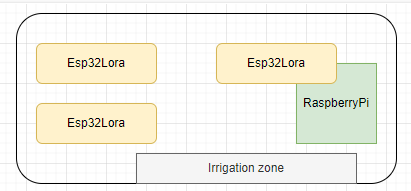
\includegraphics[width=0.8\textwidth]{images/irrigation-zone.png}
    \caption{Irrigaiton zone}
    \label{fig:irrigation-zone}
\end{figure}

\subsection{Zone Activation}

The activation process is done in the following steps:
\begin{enumerate}
    \item The user enters the code displayed on the Raspberry Pi OLED display in the web application.
    \item The web application sends the code to the web API.
    \item The web API verifies the code and activates the irrigation zone.
    \item The web API sends a message to the Iot Device to activate the irrigation zone.
    \item The Raspberry Pi receives the message from Azure IoT Hub and activates the irrigation zone.
    \item The Raspberry Pi sends a message to the ESP32 nodes to start collecting data from the sensors.
\end{enumerate}

\begin{figure}[H]
    \centering
    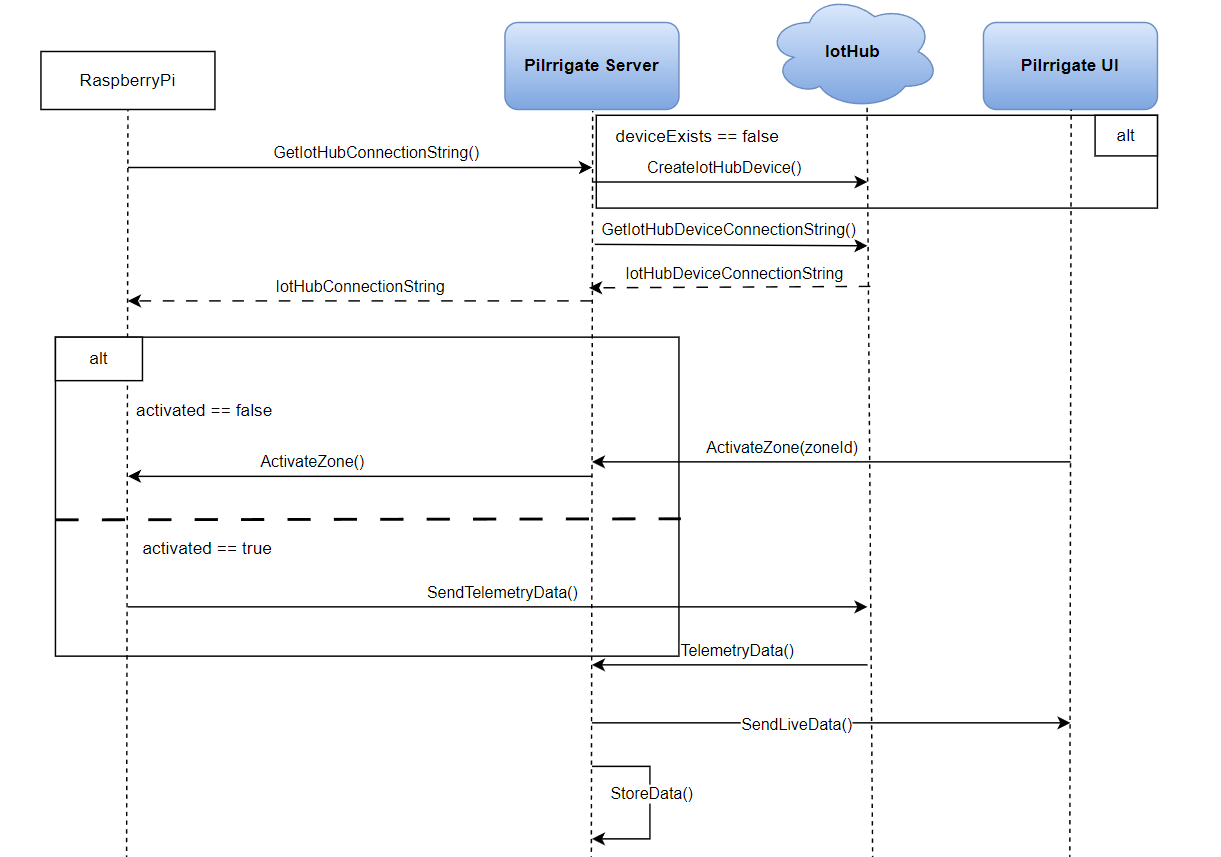
\includegraphics[width=0.9\textwidth]{images/activation.png}
    \caption{Zone activation process}
    \label{fig:zone-activation}
\end{figure}

\subsection{Web API}
The web API is developed in \.NET ans it is responsible
for user management, data storage, and communication with the IoT Hub.
It uses Entity Framework Core to interact with the 
PostgreSQL database and SignalR to provide real-time communication.
It uses the controller pattern to handle the HTTP requests. 
I created a controller for each resource in the system,
such as users, zones, data, devices, schedules and cloud to device messages.

\subsubsection{Zone Controller}
Since the first step in the activation process is to verify the code enterede by the
user, I will start describing the zone controller.
Using this controller, the user can create a zone, activate a zone, get the IoT Device connection string, retrieve
all zonees, get a zone by id, and delete a zone. For the database interaction, I created
a zone repository that implements the IZoneRepository interface.
\begin{lstlisting}[caption={Zone Repository interface}]
public interface IZoneRepository
{
    public Task<bool> CreateZone(Zone zone);
    public Task<bool> UpdateZone(Guid Id, string Name, Guid userId);
    public Task<bool> DeleteZone(Guid Id);
    public Task<Zone> GetZoneById(Guid Id);
    public Task<Zone> GetZoneByName(string name);
    public Task<IEnumerable<Zone>> GetAllByUserId(Guid Id);
}
\end{lstlisting}

The controller is also using the IoTDeviceManager service to manage the
IoT devices in Azure IoT Hub, which implement the IioTDeviceManager interface and 
is repsonsible for creating, deleting, and checking the existence of IoT devices.

\begin{lstlisting}[caption={IoT Device manager interface}]
public interface IiotDeviceManager
{
    public Task<bool> CreateIotDevice(string zoneId);
    public Task<string> GetDeviceConnectionString(string zoneId);
    public Task<bool> DeviceExists(string zoneId);
    public Task<bool> DeleteIotDevice(string zoneId);
}
\end{lstlisting}

\subsubsection{Data Controller}
The data controller is used to retrieve data from the PostgreSQL database.
It provides endpoints for:
\begin{itemize}
    \item Get all data for a zone, including the data for all devices in that zone.
    \item Get data for a certain period of time.
    \item Get all data foor a device.
    \item Get data for a device for a certain period of time.
\end{itemize}

The data controller will use the IDataService for all the logic related to data retrieval.
For the DataService, all the database interaction is done within that service.

\subsubsection{Device Controller}
The device controller is used to manage the devices in the system.
It provides endpoints for:
\begin{itemize}
    \item Get all devices for a zone.
    \item Get all devices for a user.
    \item Get a device by id.
    \item Get a device by MAC address.
    \item Register a new device.
\end{itemize}

\subsubsection{C2D Controller}
The C2D (Cloud to Device) controller is used to manage the cloud to device messages in the system.
It provides only one endpoint to send a message to a device. The endpoint accepts a C2DMesageRequest object, 
which contains the zoneId, and an object of type C2DMethodCall, which contains the the deviceId, the method name, and a list of parameters.
\begin{figure}[H]
    \centering
    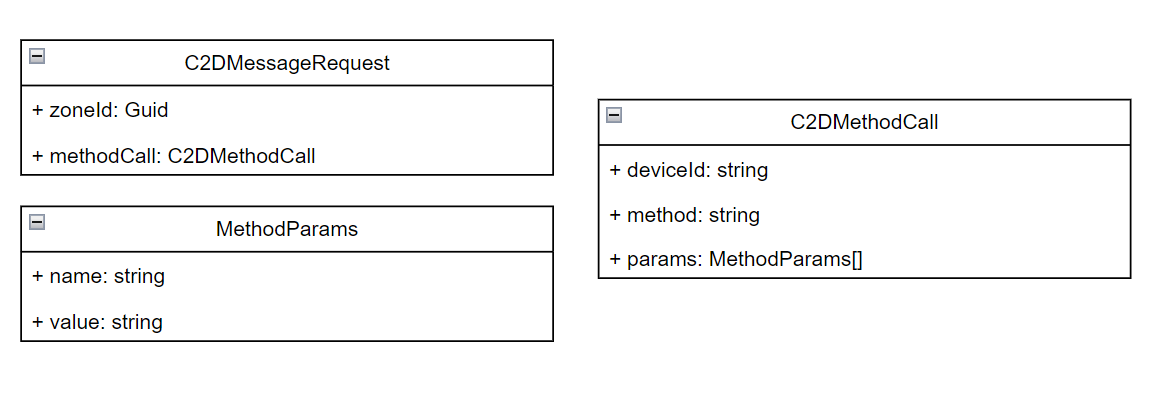
\includegraphics[width=0.8\textwidth]{images/c2d-message-request.png}
    \caption{C2D Message Request object}
    \label{fig:c2d-request}
\end{figure}

\subsubsection{Schedule Controller}
The schedule controller is used to manage the irrigation schedules in the system.
It provides endpoints for:
\begin{itemize}
    \item Get all schedules.
    \item Get a schedule by id.
    \item Create a new schedule.
    \item Update an existing schedule.
    \item Delete a schedule.
\end{itemize}

The Schedule object is defined as follows:
\begin{figure}[H]
    \centering
    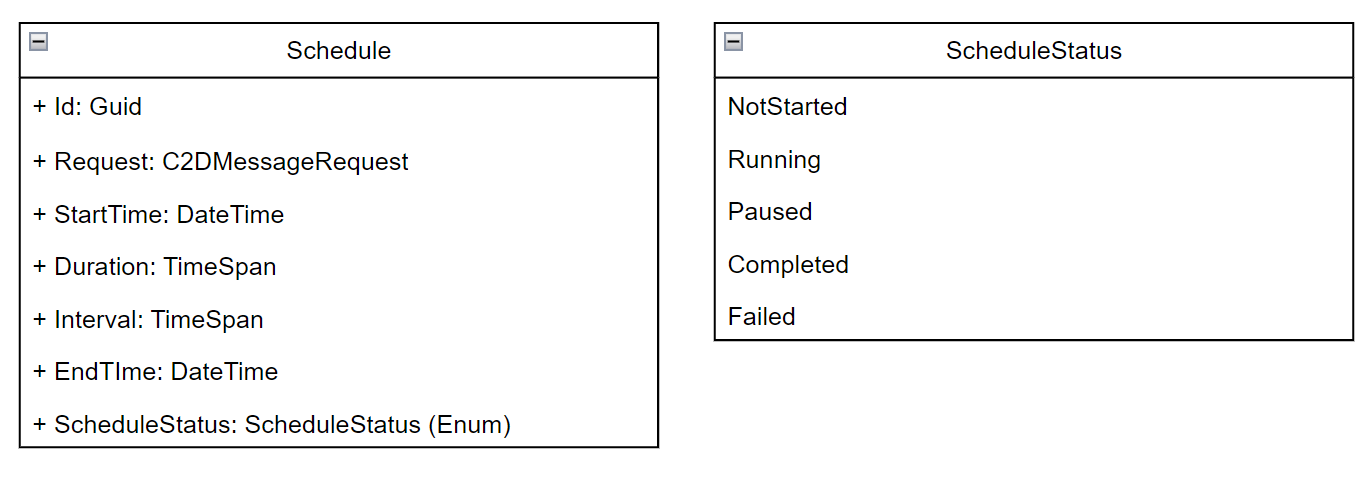
\includegraphics[width=0.8\textwidth]{images/schedule.png}
    \caption{Schedule object}
    \label{fig:schedule-object}
\end{figure}

\begin{enumerate}
    \item The Id is a unique identifier for the schedule.
    \item The Request is an object of type C2DMesageRequest that contains the zoneId, deviceId, method name, and parameters.
    \item The StartTime is the time when the schedule should start.
    \item The EndTime is the time when the schedule should end.
    \item The Interval is the time interval between two consecutive executions of the schedule.
    \item The Duration is the duration of the schedule execution.
    \item The ScheduleStatus is the status of the schedule, which can be NotStarted, Running, Paused, Completed, Failed.
\end{enumerate}

The user can create a new schedule using the UI of the web application,
which will send a request to the web API to create a new schedule. 
The web API will validate the request and create a new schedule in the database.
A bragraound service will be used to check and execute the schedules. The background service will run 
every minute and check if there are any schedules that should be executed or stoped. To be more robust, the duration 
of the schedule, as well as the start and end time, will be sent to the Raspberry Pi, wich will also check if 
the schedule should be executed or stopped. This way if the Web API or the network connectivity is down, 
the Raspberry Pi will still be able to execute the schedules.

A background service is used to check the schedules. A baground services is a service that implements
the IHostedService interface and runs tasks in the background. It is used to perform long-running tasks and
it implements the StartAsync and StopAsync methods \cite{IHostedService}.


\subsubsection{User Controller}
As the user needs to be authenticated to access the web API,
I created a user controller that handles user registration and login.

\begin{lstlisting}[caption={User Service interface}]
public interface IUserService
{
    Task<UserDto> GetUserByIdAsync(Guid userId);
    Task<IEnumerable<UserDto>> GetAllUsersAsync();
    Task<bool> UpdateUserProfileAsync(Guid userId, UpdateProfileRequest request);
    Task<bool> ChangeUserRoleAsync(Guid userId, string newRole);
    Task<AuthResult> RegisterUser(RegisterRequest register);
    Task<AuthResult> LoginUser(LoginRequest request);
}
\end{lstlisting}

For accessing the user data, UserRepository is used, which implements the IUserRepository interface.
The authorization is done using JWT tokens, 
which are generated when the user logs in. To handle all the logic related to 
JWT tokens, I created a JWT service that implements the IJwtService interface.
Besides IUserRespository, and IJwtService, the UserService is also using
IPasswordHasher to hash the user passwords. This provides abstraction
for hashing and verifying passwords, 
allowing for easy integration with different hashing algorithms. For the moment,
the implementation uses SHA256 hashing algorithm, 
but it can be easily changed to any other algorithm. In the future, I plan to replace
this with Microsoft.AspNetCore.Identity, 
which provides a more secure and flexible way to handle user 
authentication and authorization and it is widely used in the \.NET community.

\begin{lstlisting}[caption={User Repository interface}]
public interface IUserRepository
{
    Task<User> GetByIdAsync(Guid id);
    Task<User> GetByEmailAsync(string email);
    Task<IEnumerable<User>> GetAllAsync();
    Task<bool> CreateAsync(User user);
    Task<bool> UpdateAsync(User user);
    Task<bool> DeleteAsync(Guid id);
}
\end{lstlisting}

\begin{lstlisting}[caption={JWT Service interface}]
public interface IJwtService
{
    string GenerateJwtToken(User user);
    bool ValidateToken(string token);
}
\end{lstlisting}

\begin{lstlisting}[caption={Password Hasher interface}]
public interface IPasswordHasher
{
    string HashPassword(User user, string password);
    bool VerifyPassword(User user,string hashedPassword, string providedPassword);
}
\end{lstlisting}

\subsubsection{Registration Flow}
The registration flow is as follows:
\begin{enumerate}
    \item The user fills the registration form in the web application.
    \item The web application sends the request to the web API. More sdpecifically, 
    it sends a POST request to the register endpoint of the user controller. The controller
    receives the request as an object of type RegisterRequest.
    \item The request is being validated by the web API.
    \item If the request is valid, the web API creates a new user in the database
    \item The web API generates a JWT token and it sends back an object of type AuthResult.
    \item The web application receives the AuthResult object and stores the JWT token in the local storage.
\end{enumerate}

The registration flow is shown in the figure below.
\begin{figure}[H]
    \centering
    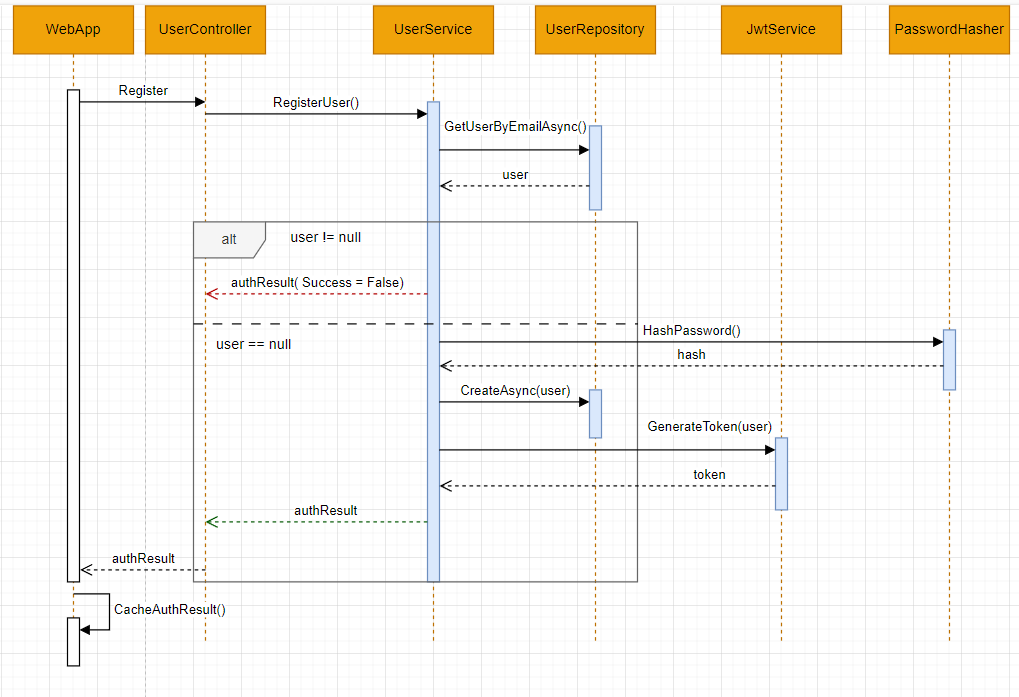
\includegraphics[width=0.9\textwidth]{images/registration-flow.png}
    \caption{Registration flow}
    \label{fig:registration-flow}
\end{figure}

The AuthResult object and the RegisterRequest object are defined as follows:
\begin{figure}[H]
    \centering
    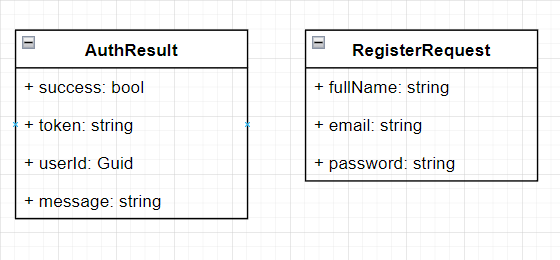
\includegraphics[width=0.8\textwidth]{images/auth-request.png}
    \caption{AuthResult and RegisterRequest objects}
    \label{fig:auth-result}
\end{figure}

\subsubsection{Login Flow}
The login flow is similar to the registration flow, but it does not create a new user.
The login flow is as follows:
\begin{enumerate}
    \item The user fills the login form in the web application.
    \item The web application sends a POST request to the login endpoint of the user controller. The controller
    receives the request as an object of type LoginRequest.
    \item The request is being validated by the web API.
    \item If the request is valid, the web API checks if the user exists in the database.
    \item If the user exists, the web API verifies the password and generates a JWT token.
    \item The web API sends back an object of type AuthResult.
    \item The web application receives the AuthResult object and stores the JWT token in the local storage.
\end{enumerate}

The login flow is shown in the figure below.
\begin{figure}[H]
    \centering
    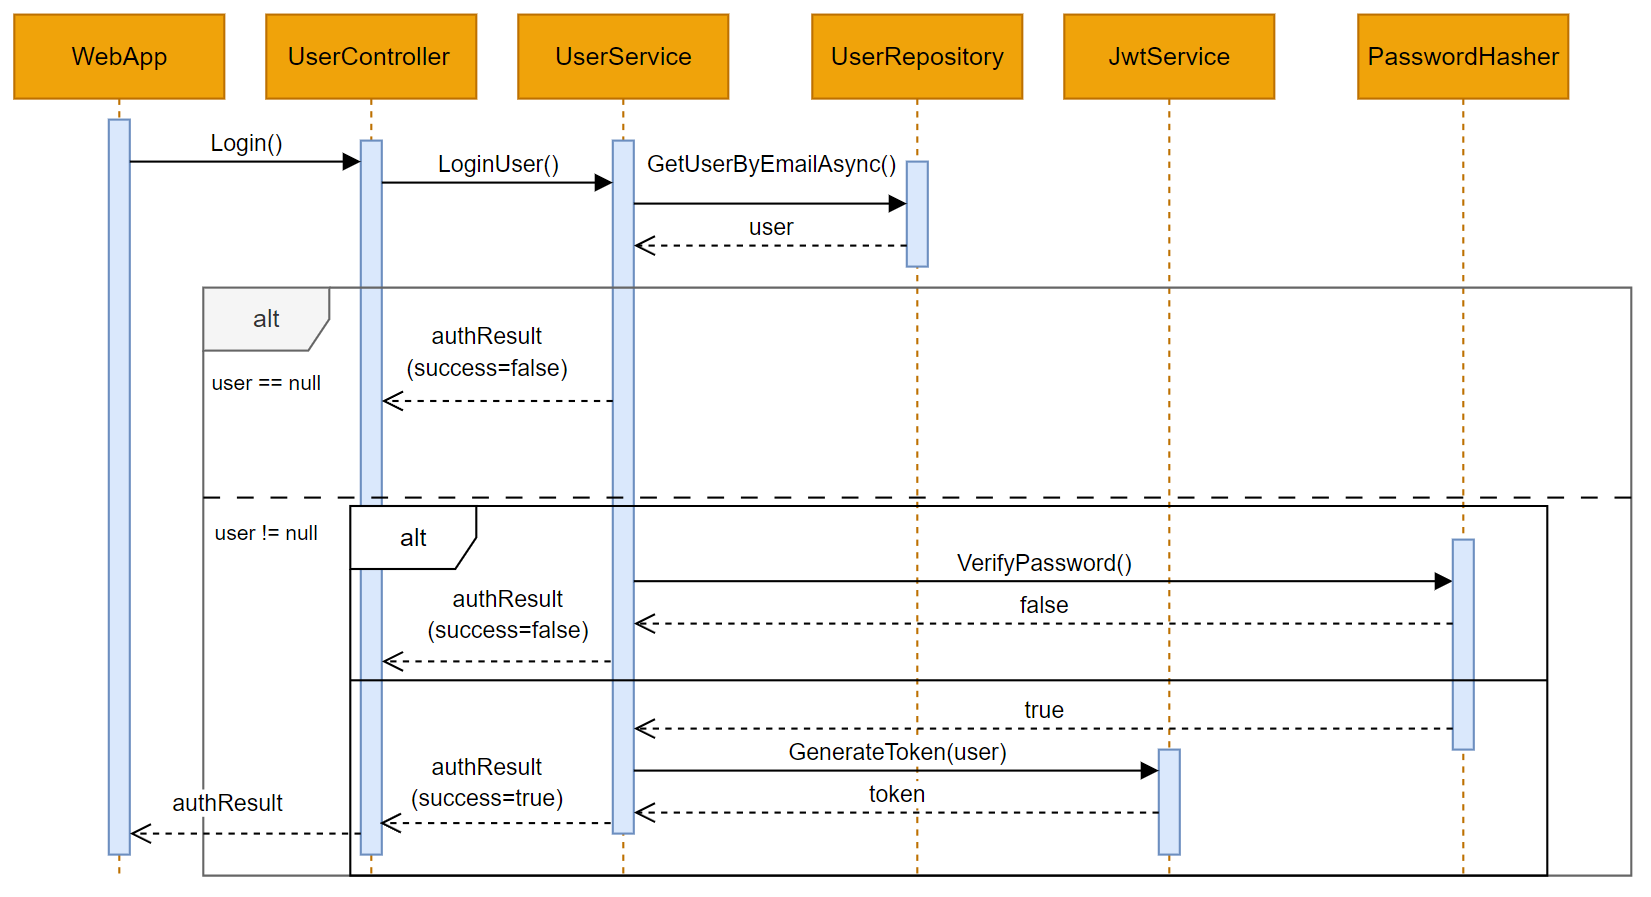
\includegraphics[width=0.9\textwidth]{images/login-flow.png}
    \caption{Login flow}
    \label{fig:login-flow}
\end{figure}

\subsection {Web Application}
The web application for this project is developed using Angular v19. Most of the UI components are 
created using Angular Material, but some of them are custom made, to fit the needs of the project.
I tried to keep the UI as simple as possible, while still providing all the necessary features.

\subsubsection{Landing Page}
When entering the web application, the user is presented with a landing page that contains information about
the PiIrrigate project and a button to register. More precisely, it contains a scrollable carousel with the 
main functionalities of the project.
The web application is designed to be responsive and
to work on both desktop and mobile devices. The landing page is shown in the figure below. In this 
figure you can see the landing page as is displayed on a desktop device.

\begin{figure}[H]
    \centering
    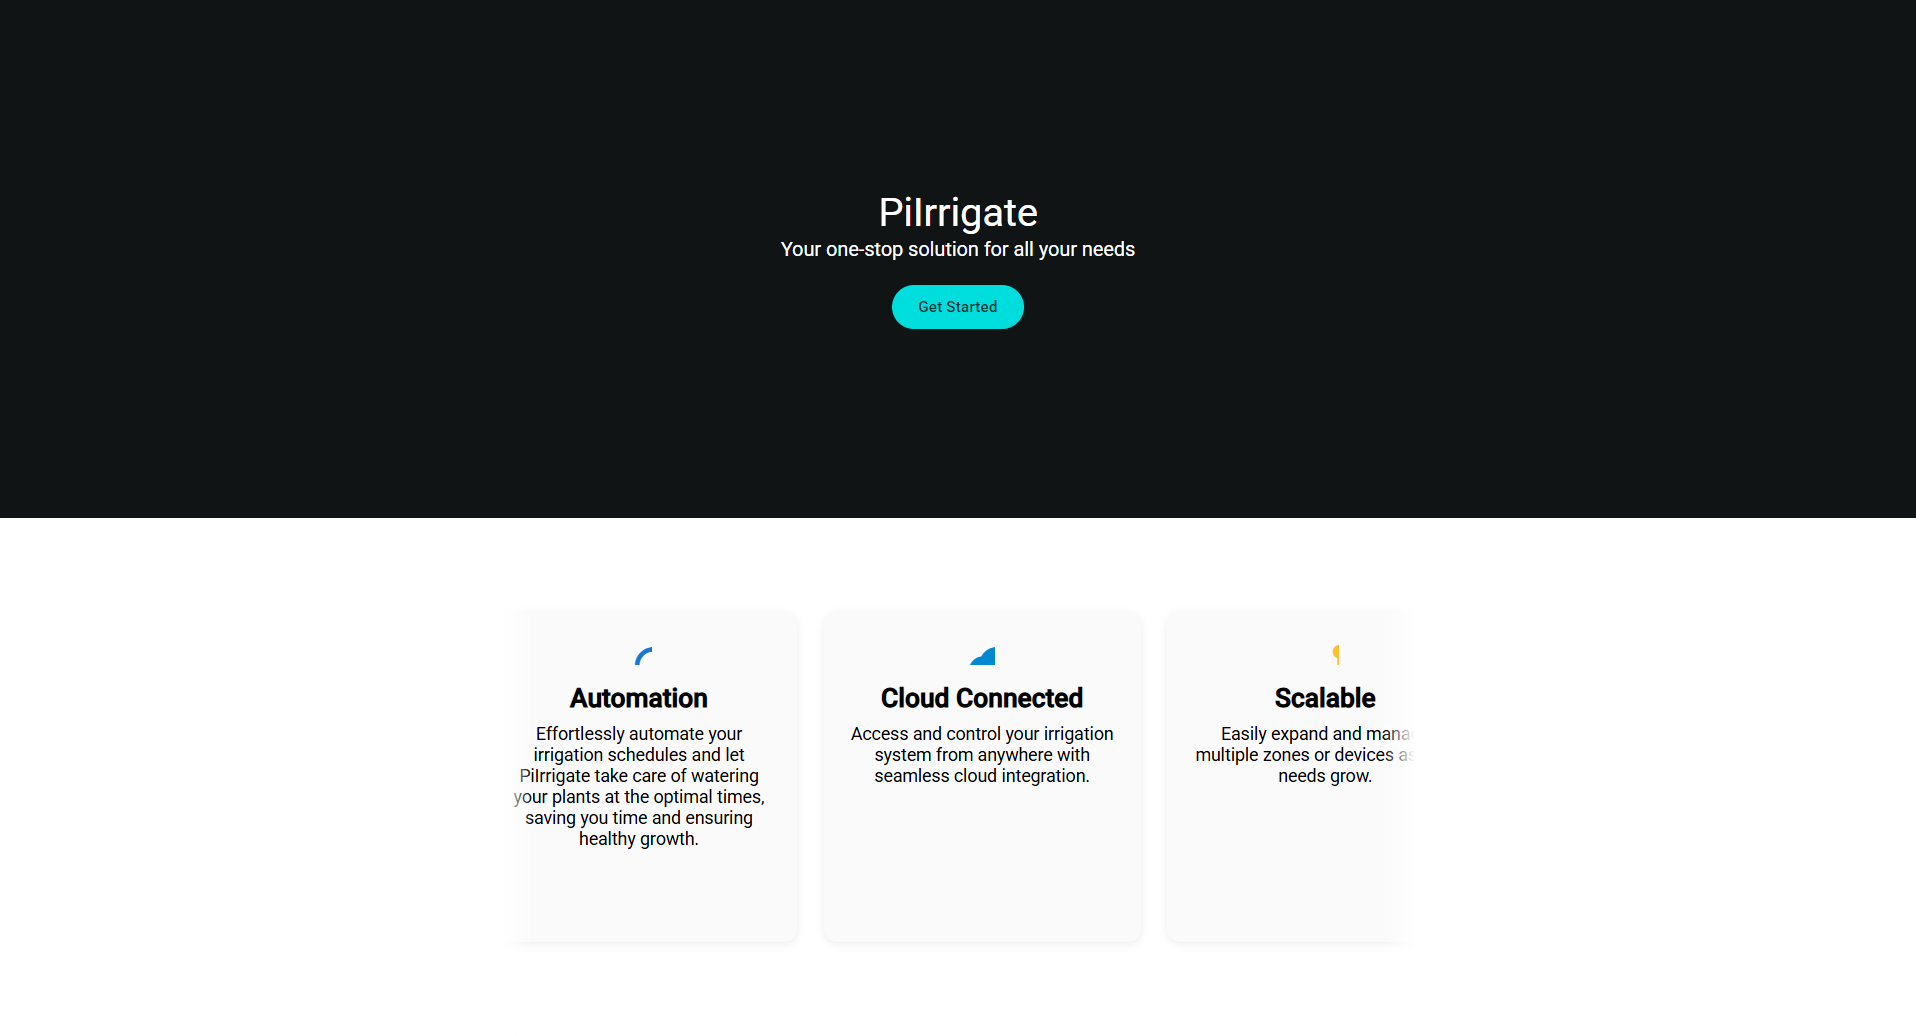
\includegraphics[width=0.8\textwidth]{images/landing_page.png}
    \caption{Landing page of the web application}
    \label{fig:landing-page}
\end{figure}

In the following figure you can see the landing page as it is displayed on a mobile device (iPhone 12 Pro).

\begin{figure}[H]
    \centering
    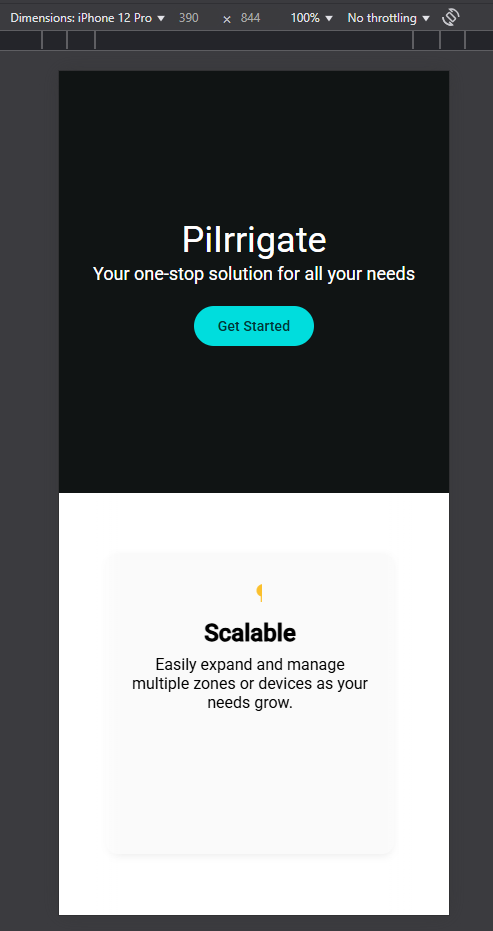
\includegraphics[width=0.6\textwidth]{images/landing_12_pro.png}
    \caption{Landing page of the web application on mobile device}
    \label{fig:landing-page-mobile}
\end{figure}

\subsubsection{Login and Registration User Flow}
Users can login or register using the login and register form.
After the user clicks on the \"GetStarted\" button from the landing page. it will be redirected to the 
register page. 
In the following figure you can see the loign and registration flow.
\begin{figure}
    \centering
    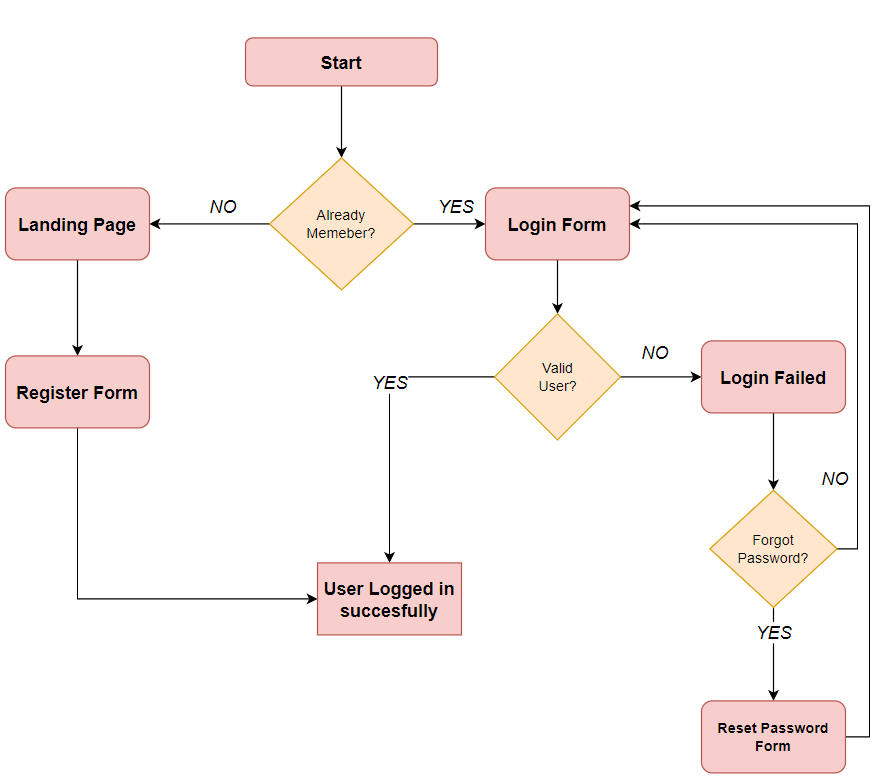
\includegraphics[width=0.9\textwidth]{images/user_flow.png}
    \caption{Login and registration user flow}
    \label{fig:login-registration-flow}
\end{figure}



\subsubsection{Login and Registration}
The login and registration pages repsect the design principles of the entire web application so 
they are siple and easy to use. 



\chapter{Conclusions}
\thispagestyle{pagestyle}

\begin{code}
	\begin{lstlisting}[language=Java]
public class Client {
	public static void main(String[] args) {
		Animal tiger = new Tiger();
		Animal parrot = new Parrot();
		tiger.breed(parrot);
	}
}
	\end{lstlisting}
	\caption{Subtype polymorphism example \cref{code:polym2}}
	\label{code:polym3}
\end{code}

The paper will end with a chapter of conclusions. It will contain the main results of the work and their practical implications. In the case of diploma projects, the main synthetic data obtained from the design process will be mentioned.

\section{Bibliography}
At the end of the paper will be given a list of references for the scientific texts consulted during the work. All sources will be listed, including those on the internet. These will be referenced in the text and listed in alphabetical order, as in the examples below.

\textbf{IMPORTANT:} Citations are not entered manually, but by using the biblatex library. References can be generated with various external tools in .bib format and then inserted into the project structure in bibliography.bib. Further reading:
\begin{enumerate}
    \item Docs: \url{https://mirrors.nxthost.com/ctan/macros/latex/contrib/biblatex/doc/biblatex.pdf}
    \item Convert DOI to .bib: \url{https://www.doi2bib.org/}
\end{enumerate}


Bibliography should include all literature titles that have served as a basis for documentation, i.e. authors who have been quoted in the text, in all chapters of the thesis paper. 

The Faculty of Automation and Computers requires the use of the IEEE citation style (details \url{https://ieee-dataport.org/sites/default/files/analysis/27/IEEE\%20Citation\%20Guidelines.pdf}), used primarily in scientific publications in the field of IT. The three important parts of the reference are:
\begin{enumerate}[leftmargin=2cm,topsep=1.15pt,itemsep=1.15pt,partopsep=1.15pt,parsep=1.15pt,label=\alph*.]
   \item The name of the author indicated as the first initial of the first name, then the full name.
   \item The title of the article, the patent, the conference paper, etc., in quotation marks.
   \item The title of the magazine or book in italics.
How the reference is written depends on the type of publication, please follow the instructions at the link above carefully.
\end{enumerate}
	 
Each citation should be noted in the text using simple sequential numbers. A number in square brackets, placed in the text of the report, indicates the specific reference. Citations are numbered in the order in which they appear. Once a source has been cited, the same number is used in all subsequent references in the text. No distinction is made between electronic and printed sources, except for the details of the cited references.


Each reference number must be enclosed in square brackets on the same line as the text, before any punctuation mark, with a space before the parentheses.

Examples:
\begin{enumerate}[leftmargin=2cm,topsep=1.15pt,itemsep=1.15pt,partopsep=1.15pt,parsep=1.15pt,label=\alph*.]
   \item ". . .the end of my research [13]."
   \item "The theory was first introduced in 1987 [1]."
\end{enumerate}

The list of references in the bibliography is composed of all the sources used to document the paper and is made in the numerical order of the citation in the text and not in alphabetical order of the authors.

The identical insertion of a sentence or paragraph shall be made by including the page from the source used, but also by quotation marks and the use of Italics; for sources taken from the Internet, the page addresses shall be included; in the final bibliographic list the works shall be entered in the alphabetical order of the authors' names. For collective works, the rule of alphabetical order applies to the first author. 

If websites, magazines or articles are quoted, three asterisks will appear before, and then information on the volume, the issue, the pages consulted, the exact website address of the article, the date of the site visit and the date of downloading, as well as the date of the accessing. Web page addresses will be entered at the end of the list.

The bibliographical sources the author of which cannot be mentioned should be specified as "***" followed by the name of the article and/or book, the publishing house and the place of appearance (for books), the volume, the issue, the first and last page of the quoted work, and the year of appearance. 

*** https://ro.wikipedia.org/wiki/Motor accessed February 2022

Example: \label{example:citation} Einstein \cite{einstein}, mentioning \enquote{The intuitive mind is a sacred gift.}

\section{Authenticity Declaration}
The last page of the thesis paper shall contain the „Statement regarding the authenticity of the thesis paper”, in handwriting, filled in according to the UPT’s requirements. The Statement shall be downloaded from the web, at:

\url{http://www.upt.ro/img/files/Regulamente_UPT/2020/Declaratie_de_autenticitate_UPT_2020.pdf}

% Look for building the .bib file on Overleaf documentation
\printbibliography[heading=bibnumbered]

\includepdf[pages={1}]{\declarationPath}

\end{document}